% First draft using the supplied Bath RL project template and unmodified style.
\documentclass[letterpaper]{article}
\PassOptionsToPackage{numbers,sort&compress}{natbib}
\usepackage[final]{rl_project}
\usepackage[T1]{fontenc}
\usepackage[utf8]{inputenc}
\usepackage{microtype}
\usepackage{amsmath,amssymb,booktabs,array,graphicx,xcolor}
\usepackage{hyperref}\hypersetup{hidelinks}
\usepackage{url}
\graphicspath{{figures/}}
\newcommand{\drafttodo}[1]{\textcolor{red!65!black}{\textbf{[Draft TODO: #1]}}}
\title{Tactical Knowledge in Connect Four Reinforcement Learning}
\author{\textit{Group names and student numbers to be added}\\
Department of Computer Science\\
University of Bath}

\begin{document}
\maketitle

\section{Problem Definition}
Connect Four is a deterministic, fully observable, zero-sum game on a $6\times7$
board. Players drop pieces into non-full columns; four connected pieces win and
a full board without a winner draws. Games last at most 42 moves.

A state $s=(B,p)$ records the board and player to move. Legal actions are non-full
columns, and $T(s,a)$ applies gravity and switches players. Rewards are zero
until termination: $z=+1$ for a win, $-1$ for a loss and $0$ for a draw, without
discounting. For a fixed pair of policies $\mu$, the player-to-move value is
\begin{equation}
 V^\mu(s)=\mathbb E_\mu[z\mid s]
 =-\sum_{a\in\mathcal A(s)}\mu(a\mid s)V^\mu(T(s,a))
 \quad\text{for non-terminal }s.
 \label{eq:bellman}
\end{equation}
Terminal values are exact outcomes; the minus sign accounts for alternating
players~\cite{sutton2018}. Self-play changes the opponent distribution, so this
is not a stationary fixed-opponent learning problem.
Appendix~\ref{app:mathematics} specifies the return and minimax conventions.

Although solved, Connect Four has approximately $4.53\times10^{12}$ legal
positions~\cite{tromp}. A dense table of seven float32 action values per position would occupy about 127~TB before symmetry reduction.
A finite-horizon game permits exact late-game checks~\cite{allis1988}. The coursework permits previously solved tasks that require function approximation~\cite{brief}.
We ask how well a Q-network learns from fresh weights, whether tactical
supervision or longer temporal-difference targets improve greedy play,
and whether learned values improve a fixed search. The inherited search
agent provides a deployment benchmark.

\section{Background}
Temporal-difference self-play learned strong backgammon policies in
TD-Gammon~\cite{tesauro1995}. DQN adds replay and a delayed target
network~\cite{mnih2015}; Double DQN separates selecting and assessing a
successor action~\cite{vanhasselt2016}. In an alternating zero-sum game, the
successor's selection error enters the mover's target with a negative sign.
PPO offers a policy-gradient alternative with a different data
budget~\cite{schulman2017}.

Auxiliary losses can improve the representations available to an RL
agent~\cite{jaderberg2016}. We supervise the same action values with
short, exact tactical outcomes. Connect Four solvers also exploit immediate
losing replies to prune search~\cite{pons-tactics}. The supervised labels
and the inference filter use that information at different stages.

UCT allocates simulations through bandit exploration~\cite{kocsis2006}.
AlphaGo and AlphaGo Zero combine networks and search~\cite{silver2016,silver2017zero}.
AlphaZero and Expert Iteration use search to generate stronger policy
targets~\cite{silver2018,anthony2017}. KataGo and Gumbel planning improve
search efficiency~\cite{wu2019,danihelka2022}, while Go-Exploit addresses
coverage directly in Connect Four~\cite{trudeau2023}. Fixed opponents and
multiple training seeds help separate policy improvement from shifting
self-play populations~\cite{lanctot2017,henderson2018,agarwal2021}.
Appendix~\ref{app:literature} gives the broader review.

\section{Method}
\subsection{Implementation provenance}
Our PyTorch DQN, Double DQN, tactical loss and evaluator use the upstream
board environment. The inherited comparison
uses Eugene Peng's residual policy--value model, MCTS and pretrained
checkpoint at commit \texttt{a936aadd74a6}~\cite{peng}. We extended its
training controller, search implementation and Kaggle export. The source
archive identifies inherited and newly written paths. Appendix~\ref{app:reproducibility}
records configuration and evidence locations.

\subsection{Double DQN from fresh weights}
Double DQN~\cite{mnih2015,vanhasselt2016} starts from fresh weights and learns
seven action values from three binary planes for current pieces, opposing pieces,
and player identity. Two $3\times3$
convolutions with 32 channels and ReLU feed a 128-unit ReLU layer and seven
tanh outputs. Inference takes the highest-valued legal column in one forward pass.

The one-step baseline stores single-move transitions. The mover receives $r=1$ for a winning move
and zero otherwise. For a live successor, the target is
\begin{equation}
 y=r-Q_{\bar\theta}(s',a^*),\qquad
 a^*=\arg\max_{b\in\mathcal A(s')} Q_\theta(s',b).
 \label{eq:ddqn}
\end{equation}
The minus sign converts the opponent's return to the mover's perspective.
For a terminal successor $y=r$, including zero for a draw. The finite horizon
allows an undiscounted target. The DQN control uses the frozen target network
$Q_{\bar\theta}$ for selection as well as evaluation. Maximisation error in
the successor estimate enters the mover's target with the opposite sign.

Both players use the same $\epsilon$-greedy learner. Exploration decays linearly
from 1.0 to 0.05. A 50,000-move replay buffer supplies uniform batches of 128.
Starting at 1,024 moves, one Huber-loss update runs every four moves with Adam
($3\times10^{-4}$) and gradient norm clipping at 1.0. The target network is
copied every 500 updates. Unit checks cover terminal rewards, legal masks,
the sign of the update, and target synchronisation.

The initial study pairs DQN and Double DQN across seeds 51--53 at 5,000
games per run. It motivated a follow-up with training budgets in moves
(Appendix~\ref{app:q-study}).

To test credit assignment, we compare one-step and up-to-three-step targets~\cite{hessel2018}.
Both arms use plain Double DQN, 80,000 moves and 19,745 updates per seed.
Multi-step targets alternate the reward and bootstrap signs and stop at
termination or before a later exploratory draw. The final contrast pools
ten paired initialisations. Appendix~\ref{app:final-controls} describes the
replication and realised horizon distribution.

\subsection{Tactical supervision and inference}
Let $C(s)$ contain legal actions with an exact one- or two-ply certificate
$g(s,a)$. A terminal move yields its exact outcome ($+1$ or $0$).
Giving the opponent a winning reply certifies $-1$. Other actions remain
unlabelled. With unit Huber loss $h$, we train with
\begin{equation}
 \begin{aligned}
 \mathcal L={}&\frac{1}{|\mathcal B|}\sum_{i\in\mathcal B}h(Q_\theta(s_i,a_i)-y_i)\\
 &\quad+\frac{\lambda}{\max(1,M)}\sum_{i\in\mathcal B}\sum_{a\in C(s_i)}
     h(Q_\theta(s_i,a)-g(s_i,a)).
 \end{aligned}
 \label{eq:tactical-loss}
\end{equation}
$M$ counts certified actions across the batch. The control uses $\lambda=0$ and the treatment uses $\lambda=1$. The original study pairs
five initialisations (seeds 61--65) at 80,000 moves and 19,745 updates per
run. Exploration decays over 64,000 moves. Both policies generate their
own self-play. Greedy inference uses one network call. For an inference
ablation, a tactical filter takes an immediate win or rules out moves
allowing an immediate loss if a safe move exists. The tactics-only baseline
samples uniformly from the filtered choices.

\subsection{Evaluation and search reference}
Game score is $S=(W+D/2)/n$. We pair games by opening and swap seats for
each opening. Curves use 24 openings. The primary comparison uses the
80,000-move greedy checkpoints on 64 separate openings against depth-two
minimax, with a depth-three check on the first 32. Opening sets exclude
earlier evaluation boards and their reflections. Intervals across paired
seed differences address training variation. Resampled opening intervals
condition on the trained runs. Evaluating games may revisit positions seen
during self-play.

The 288 exact endgames comprise 96 immediate wins, 96 defensive choices
and 96 multi-step positions with different action outcomes. For the latter,
the tactical certificates give no action label. We solve each legal action
to the end, independently verify its value, and credit selection of any
optimal move. The fixed puzzle mix supports diagnosis of three abilities.

After a 24-opening pilot, we freeze 128 new opening pairs. The primary
search comparison holds the two-ply tree fixed and changes only the leaves
from a hand-coded window heuristic to learned Q-values. Its opponent is
depth-three minimax. The horizon comparison uses greedy play against
depth-two minimax on the same set. The defensive diagnostic gives both
networks the same match positions and their reflections. These three
controls each use ten seeds after a five-seed replication. We report
mean $\pm$ sample SD across seeds and keep confidence intervals separate.

The inherited search reference retains its pretrained weights. We compare
its greedy policy prior with 64 PUCT simulations on the same puzzles.
Separately, our continued-training system uses 512 simulations per move
and tracks a gated champion. Its Kaggle export combines the network,
budgeted search and tactical checks. Figure~\ref{fig:inference} and
Appendix~\ref{app:search-study} document those components.

\begin{figure}[!htbp]
\centering
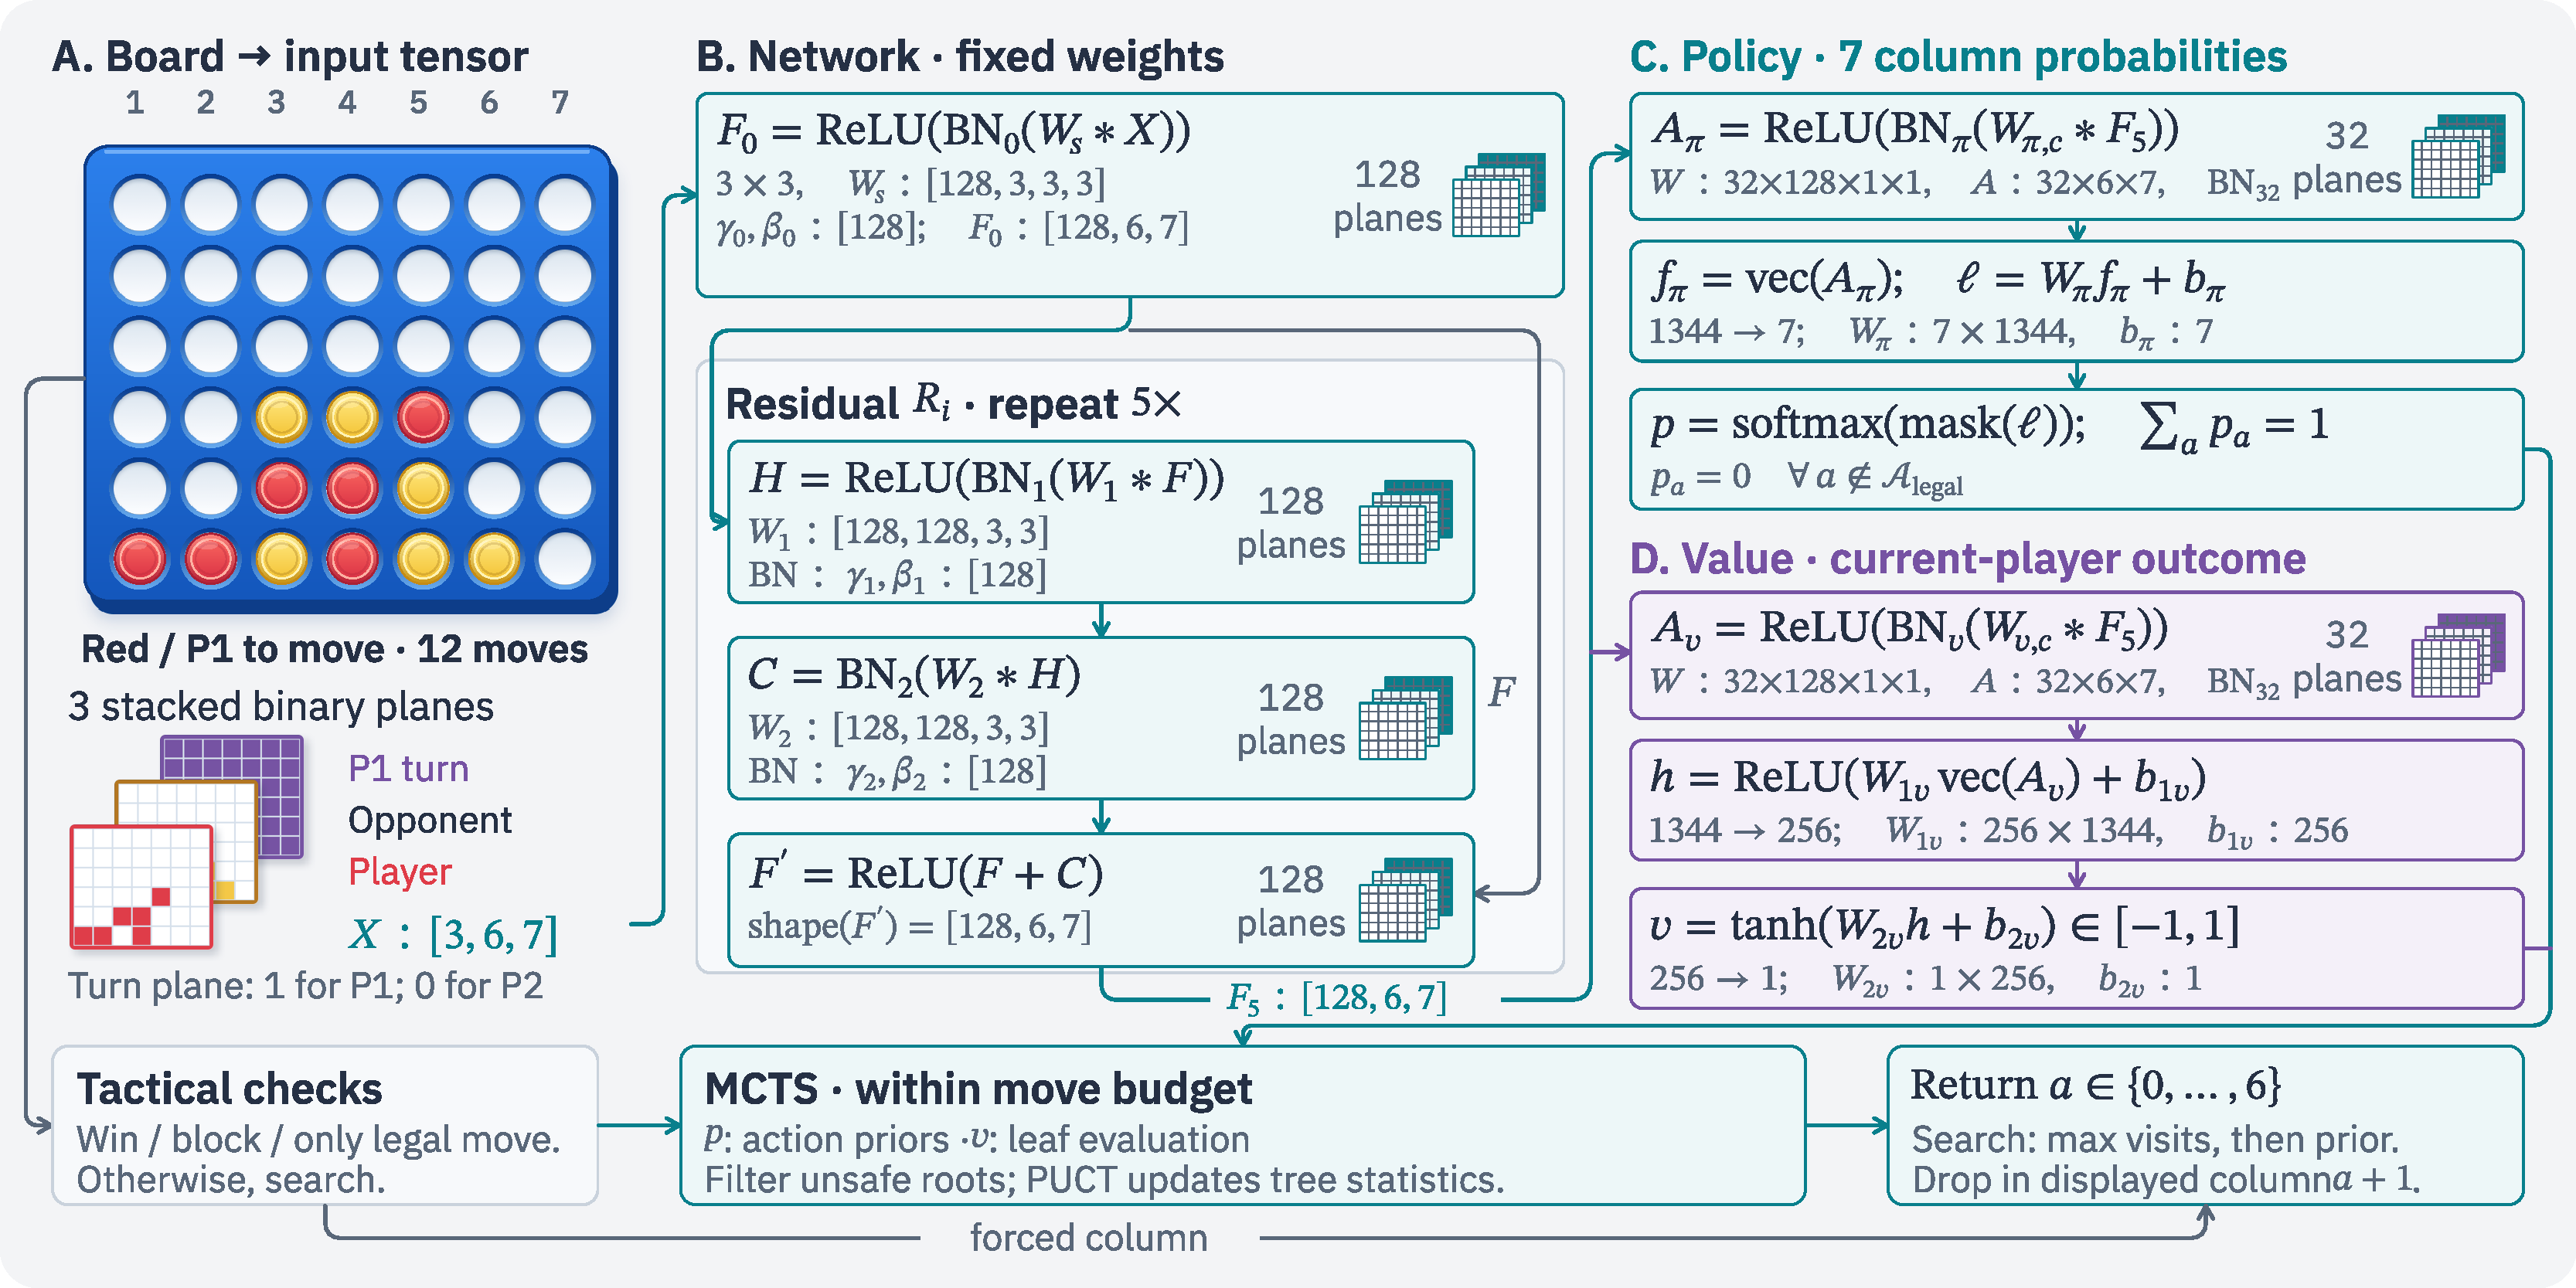
\includegraphics[width=\linewidth]{network-architecture.pdf}
\caption{Inherited search-agent deployment: board encoding, policy--value inference and move selection.
Tactical checks precede budgeted MCTS.}
\label{fig:inference}
\end{figure}

\section{Results}
\subsection{Learning with terminal rewards}
In the three-seed comparison, mean held-out greedy scores rose from
70.3\% at initialisation to 94.8\% (DQN) and 95.1\% (Double DQN) against
uniform random play. Against depth-two minimax they rose from 0.5\% to
10.9\% and 10.7\%, respectively. The paired differences change sign across
seeds. Guarding the trained networks raised both minimax scores to 27.2\%;
a tactics-only policy scored 18.8\%. The seed-51 pilot (Appendix~\ref{sec:ddqn-pilot})
found that 53 of 60 final minimax losses followed a move with a safer alternative.
Figure~\ref{fig:q-study} shows the learning curves and Appendix~\ref{app:q-study} gives the seed-level results.

\subsection{Learning to choose safer moves}
\label{sec:tactical-study}
The original ten runs generated 800{,}000 moves. On the primary test, the tactical network scored 9.8\%, compared with 11.9\% for the control. The paired difference was -2.0 percentage points (95\% seed-paired $t$ interval [-4.6, +0.5] pp; the tactical variant led in 0/5 pairs and tied 2/5). In those match traces, the greedy control exposed itself to an avoidable immediate loss on 429/1199 defensive decisions (35.8\%), compared with 438/1125 (38.9\%) for tactical supervision. Figure~\ref{fig:tactical-study} relates the learning curves to the solved-position tests.

On 1,797 shared defensive positions before move 30,
the plain and tactical networks allowed an avoidable immediate loss at
$(38.3\pm1.6)\%$ and $(42.9\pm1.4)\%$. The paired difference
was $+4.5\pm2.0$ points (95\% seed interval
$[+3.1,+6.0]$). On the solved immediate-defence set, the
original five pairs chose optimal actions at rates of 46.9\% and 51.7\%.
On multi-step puzzles those rates were 53.1\% and 50.8\%, compared with
77.1\% for the inherited prior and 93.8\% with 64 PUCT simulations.
Appendix~\ref{app:tactical-study} gives the full puzzle results.

\begin{figure}[!htbp]
\centering
\begin{minipage}[t]{.482\linewidth}
\vspace{0pt}
\centering
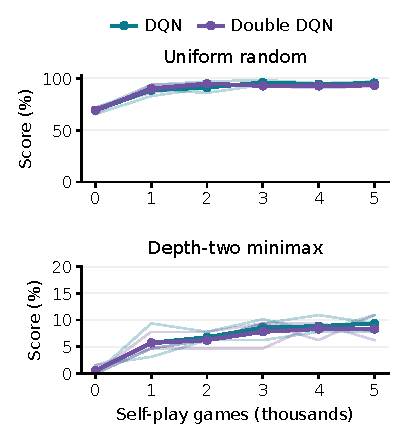
\includegraphics[width=\linewidth]{dqn-study-inline.pdf}
\caption{Initial DQN comparison. Each checkpoint uses 32 opening pairs per
seed. Thin lines show seeds and thick lines show their means. Final scores
use separate openings.}
\label{fig:q-study}
\end{minipage}\hfill
\begin{minipage}[t]{.482\linewidth}
\vspace{0pt}
\centering
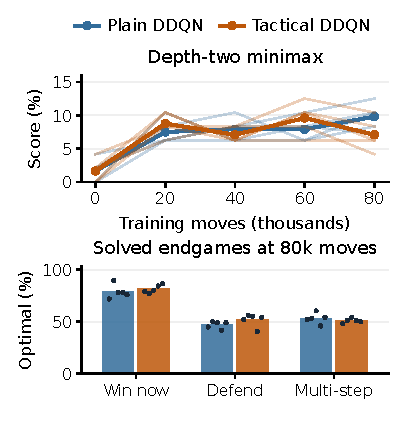
\includegraphics[width=\linewidth]{tactical-followup-inline.pdf}
\caption{Move-matched follow-up. Lines show greedy play against depth-two
minimax. Bars show mean optimal action rates on solved positions and dots
show individual seeds.}
\label{fig:tactical-study}
\end{minipage}
\end{figure}

\begin{table}[!htbp]
\centering\small
\caption{Final holdout scores, averaged over five matched seeds for learned agents. The depth-three opponent uses a common 32-opening subset. Other opponents use 64 openings. Each opening is played in both seats. Dashes indicate unevaluated cells.}
\label{tab:tactical-final}
\begin{tabular}{@{}lrrr@{}}
\toprule
Policy & Random & Minimax 2 & Minimax 3\\
\midrule
Random weights & 70.9\% & 1.0\% & --\\
Plain Double DQN & 94.1\% & 11.9\% & 11.6\%\\
Plain Double DQN + guard & -- & 27.2\% & 22.7\%\\
Tactical supervision & 94.5\% & 9.8\% & 10.9\%\\
Tactical supervision + guard & -- & 21.6\% & 23.6\%\\
Tactics only & 97.7\% & 10.9\% & 20.3\%\\
\bottomrule
\end{tabular}
\end{table}

\subsection{Learning and depth-limited search}
With the two-ply tree fixed, training changed the score by $+14.1\pm4.7$
points (95\% seed interval $[+10.7,+17.4]$). Against the hand-coded
heuristic, the trained Q evaluator differed by $-9.0\pm1.7$ points
($[-10.2,-7.8]$). With identical trained weights, moving from guarded
greedy to two plies changed the score by $+4.3\pm2.8$ points
($[+2.3,+6.3]$). Table~\ref{tab:lookahead} gives the four policies.

\begin{table}[!htbp]
\centering\small
\caption{Scores against depth-three minimax on 128 openings in both seats. Learned rows show mean $\pm$ SD across ten seeds. The window heuristic is one fixed policy.}
\label{tab:lookahead}
\begin{tabular}{@{}lr@{}}
\toprule
Inference policy & Score\\
\midrule
Initial Q-values, two-ply & $(16.4\pm4.5)\%$\\
Trained Q-values, guarded greedy & $(26.2\pm3.3)\%$\\
Trained Q-values, two-ply & $(30.4\pm1.7)\%$\\
Window heuristic, two-ply & 39.5\%\\
\bottomrule
\end{tabular}
\end{table}

\subsection{Learning with longer targets}
Against depth-two minimax, greedy one-step Double DQN scored
$(10.9\pm0.9)\%$. The up-to-three-step variant scored
$(9.7\pm0.9)\%$. The paired gap was $-1.1\pm1.4$ points.
The 95\% interval was $[-2.1,-0.1]$ on the fixed openings and
$[-2.8,+0.5]$ when varying both seeds and
openings. Three-step returns comprised 16.6\% of treatment
replay samples. Appendix~\ref{app:final-controls} gives the run-level results.

\subsection{Search-agent deployment}
Continued training stopped at 1,000,000 self-play games after 2,613 raw iterations. The persistent phase recorded 30 promotions and ended with candidate 2353 as champion. Across 29 fixed-original tests, candidate 1667 has the highest score at 62.1\% (paired 95\% interval 56.2--68.4\%). The descriptive trend is $+0.31$ percentage points per 100 candidates (95\% interval $0.08$ to $0.52$).

Figure~\ref{fig:evaluation} and Appendix~\ref{app:benchmarks} give the complete
series. Appendices~\ref{app:losses} and~\ref{app:diagnostics} show the
optimisation and player-assignment diagnostics. The team reports a \textbf{first-place Kaggle leaderboard position}
on 19 November 2026. \drafttodo{Supply the exact score, account and
submission record for this reported rank.}

\begin{figure}[!htbp]
\centering
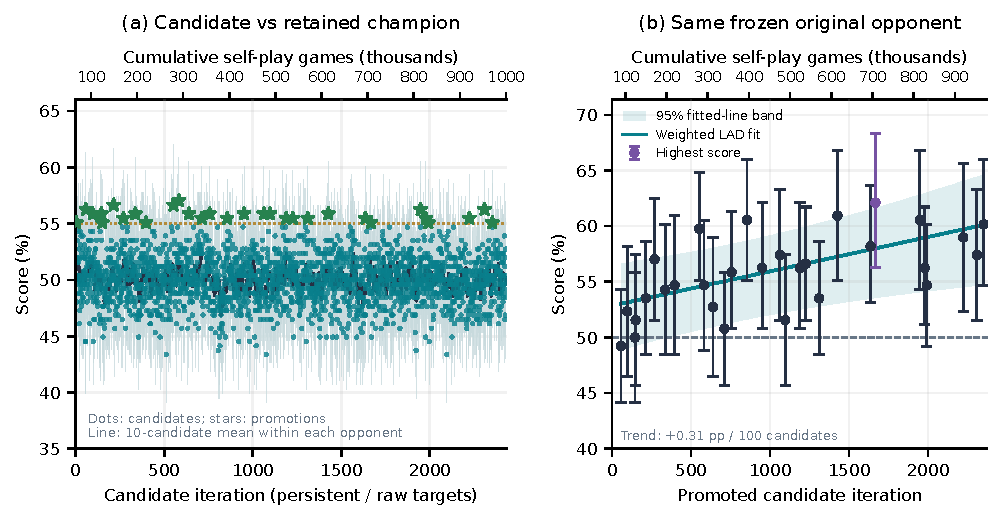
\includegraphics[width=\linewidth]{evaluation.pdf}
\caption{(a) Candidates versus the changing champion with 512 simulations per move, through final candidate 2430 (21 November, 08:17 GMT).
(b) Exported models versus the frozen original,
using 1.9-second budgets; updated 21 November, 05:59 GMT. Whiskers are paired
95\% intervals; (b) adds a weighted absolute-error fit and pointwise 95\% band.
The top axes show cumulative completed self-play games at each candidate.
Candidate 0 is original log iteration 183 (66,944 games).}
\label{fig:evaluation}
\end{figure}

\section{Discussion}
The tactical match-score interval includes zero. The tactical model
exposed itself more often even on the same positions. These positions
are conditional on facing a blockable threat against depth-two minimax.
Of 2,324 such decisions in the traces, 2,290 occurred before move 30.
The solved positions start later and use a different sampling method.
The exploratory late-game comparison uses the same exposure metric and
estimates a smaller, uncertain effect in the other direction.

The guard changes the tactical network's mean depth-two score by +11.8 points. The guarded network differs from tactics only by +10.7 points. Table~\ref{tab:tactical-final} separates this software effect from the trained network's greedy performance. Late-game labels test move quality under perfect continuation. The stratified puzzle rates depend on the imposed mix, and the match scores depend on the opponent's heuristics.

The fixed tree exposes a remaining gap to simple window counts even after
learning improves the leaf evaluator. The horizon test mixes different
bootstrap lengths, with most targets using one step under the exploration
cutoff. Its result applies to that rule and this training budget.

The search reference starts from pretrained
weights. Its internal opponents change with promotion, whereas the external
benchmark freezes the original. Reusing openings and selecting checkpoints make the intervals descriptive. Candidate 2353 scored $-2.0$ percentage points relative to candidate 1667 on the shared openings (paired 95\% interval $-8.6$ to $4.7$). Kaggle assesses the
full exported system. Its ranking alone cannot identify the effect of
continued training or of any single component.

\section{Future Work}
Test smaller tactical loss weights and compare horizon rules at matched
exploration rates. Evaluate against a wider opponent suite and, where
solving is feasible, sample earlier boards. Measure the inference latency
of each leaf evaluator with the tree fixed.

\section{Personal Experience}
\drafttodo{Each member must supply and verify their own contribution and reflection.}

The experiments offer examples for individual reflection, including CPU
search profiling, persistence across failed promotions and fixed-opponent
evaluation. Appendix~\ref{app:remaining} lists the remaining submission checks.
\label{main-text-end}

\clearpage
\section*{Generative AI Use Declaration}
OpenAI Codex/ChatGPT assisted extensively with literature searches, experiment
code, remote training, debugging, validation, log analysis, figures, submission
packaging and this report's prose and LaTeX. Codex also assisted with the
separate Q-learning implementations, tactical study, independent solver check and
agent demonstration video. Third-party code and weights are
acknowledged separately in Section 3.1 and \texttt{NOTICE}.

Automated checks do not replace human review.
\drafttodo{Each member must verify the claims, citations and implementation,
and disclose their individual GenAI use. Human review is not asserted as complete.}

\begingroup\small
\setlength{\bibsep}{1pt plus 0.4pt}
\bibliographystyle{unsrtnat}
\bibliography{references}
\endgroup

\clearpage
\section*{Appendices}
\appendix
\section{Mathematical Specification and Derivations}
\label{app:mathematics}
Indices $j,t,k$ denote moves, training cycles and optimiser steps.
The policies are unrestricted network output $p_\theta$, legal search prior
$P_\theta$, stored visit target $\pi$ and behaviour $\mu_\tau$.
The diagrams' search-path $p$ denotes $P_\theta$; their loss uses $p_\theta$.

\subsection{Game, return and value conventions}
\label{app:game-math}
Let $B_{r,c}\in\{0,1,2\}$, with $r=0$ the bottom row, and let $i\in\{1,2\}$
be the player to move. For a non-terminal state $s=(B,i)$,
\begin{equation}
 \mathcal A(s)=\{c\in\{0,\ldots,6\}:B_{5,c}=0\},\qquad
 r_c=\min\{r:B_{r,c}=0\}.
 \label{eq:legal-transition}
\end{equation}
Transition $T(s,c)$ places $i$ at $(r_c,c)$ and switches the player to $3-i$.
Terminal states have no actions. Each move adds one piece, bounding episodes at
42 plies.

Write $w\in\{1,2,\varnothing\}$ for the winner, where $\varnothing$ denotes a draw.
The utility to a fixed player $i$ is
\begin{equation}
 u_i(w)=\mathbf 1\{w=i\}-\mathbf 1\{w=3-i\},\qquad u_1(w)=-u_2(w).
 \label{eq:utility}
\end{equation}
The transition reward $r_i(s,a,s')$ is zero unless $s'$ terminates the game, when
it equals $u_i(w)$. With terminal time $H$ and $\gamma=1$, the return to the
player $i_j$ recorded at move $j$ is
\begin{equation}
 G_j^{(i_j)}=\sum_{\ell=j}^{H-1}\gamma^{\ell-j}
 r_{i_j}(s_\ell,a_\ell,s_{\ell+1})=u_{i_j}(w)=z_j.
 \label{eq:mc-return}
\end{equation}
Wins give alternating positive and negative targets; draws give zeros.
The finite horizon permits undiscounted returns without implying the contraction
properties of a discounted stationary MDP.

For fixed $\mu=(\mu_1,\mu_2)$, let
$V^\mu(s)=\mathbb E_\mu[u_i(w)\mid s=(B,i)]$.
Conditioning on the next move and using $u_i=-u_{3-i}$ gives
Equation~\eqref{eq:bellman}. Terminal nodes carry boundary value $u_i(w)$;
adding a terminal transition reward as well would count the outcome twice.
The equivalent reward-on-transition convention sets terminal continuation to zero.

For optimal adversarial play the corresponding negamax recursion is
\begin{equation}
 V^*(s)=\max_{a\in\mathcal A(s)}[-V^*(T(s,a))]
 \label{eq:negamax}
\end{equation}
at non-terminal states, with the same terminal boundary. Sign reversal implements
opposing objectives; finite neural search approximates this recursion.

For any fixed state and continuation policy, let $p_W,p_D,p_L$ be its outcome
probabilities for the player being evaluated. Then
\begin{equation}
 V=p_W-p_L,\qquad
 S=p_W+\tfrac12p_D=\frac{1+V}{2},\qquad
 p_W=\frac{1+V-p_D}{2}.
 \label{eq:value-score}
\end{equation}
Thus $(1+v_\theta)/2$ estimates score when calibrated to the evaluated policies
and states; draw probability is also needed to recover win probability.

\subsection{Forward map and parameter accounting}
\label{app:network-math}
The input $X\in\{0,1\}^{3\times6\times7}$ is
\begin{equation}
 X_{0,r,c}=\mathbf1\{B_{r,c}=i\},\quad
 X_{1,r,c}=\mathbf1\{B_{r,c}=3-i\},\quad
 X_{2,r,c}=\mathbf1\{i=1\}.
 \label{eq:encoding}
\end{equation}
The identity plane indicates whether the player to move is the first player.
Define $\rho(x)=\max(0,x)$,
$C_{a\to b}^{q}$ as a bias-free $q\times q$ convolution from $a$ to $b$ channels,
and $\mathcal B$ as channel-wise batch normalisation. All $3\times3$ convolutions
use stride one and zero padding one. The stem and five residual blocks are
\begin{align}
 F_0 &=\rho\bigl(\mathcal B_0(C_{3\to128}^{3}(X))\bigr),\\
 F_b &=\rho\!\left(F_{b-1}+\mathcal B_{b,2}\!\left(
 C_{b,2}^{3}\!\left(\rho(\mathcal B_{b,1}(C_{b,1}^{3}(F_{b-1})))\right)
 \right)\right),\quad b=1,\ldots,5.
 \label{eq:residual-map}
\end{align}
Each block convolution maps 128 channels to 128, so all $F_b$ have shape
$128\times6\times7$ and the addition is dimensionally valid. Separate
$1\times1$ convolutions define the two flattened head inputs
\begin{equation}
 h_P=\operatorname{vec}\rho(\mathcal B_P(C_{128\to32}^{1,P}(F_5))),\qquad
 h_V=\operatorname{vec}\rho(\mathcal B_V(C_{128\to32}^{1,V}(F_5))),
 \label{eq:head-features}
\end{equation}
where $h_P,h_V\in\mathbb R^{1344}$. The outputs are
\begin{equation}
 \ell_\theta=W_Ph_P+b_P,\qquad
 v_\theta=\tanh\!\left(w_V^\top\rho(W_Vh_V+b_V)+b_o\right).
 \label{eq:heads}
\end{equation}
Here $W_P\in\mathbb R^{7\times1344}$, $W_V\in\mathbb R^{256\times1344}$ and
$w_V\in\mathbb R^{256}$. Dense layers have biases. These operations follow
\path{src/neural_net/model.py} and the residual construction of He et al.~\cite{he2016}.

With frozen running mean $\bar m_c$ and variance $\bar v_c$, each BN channel is
\begin{equation}
 \mathcal B(x_c)=\gamma_c\frac{x_c-\bar m_c}
 {\sqrt{\bar v_c+10^{-5}}}+\beta_c.
 \label{eq:frozen-bn}
\end{equation}
The affine parameters $\gamma_c,\beta_c$ remain trainable; running moments and
batch counters are fixed buffers.

\begin{table}[htbp]
\centering\small
\caption{Trainable parameter accounting, including BN affine terms and dense
biases. Convolutions have no biases; running BN statistics are excluded.}
\label{tab:parameters}
\begin{tabular}{@{}lrr@{}}
\toprule
Component & Calculation & Parameters\\
\midrule
Stem & $3\cdot128\cdot9+2\cdot128$ & 3,712\\
Five residual blocks & $5\cdot2(128^2\cdot9+2\cdot128)$ & 1,477,120\\
Policy head & $128\cdot32+64+1344\cdot7+7$ & 13,575\\
Value head & $128\cdot32+64+1344\cdot256+256+256+1$ & 348,737\\
\midrule
Total & & 1,843,144\\
\bottomrule
\end{tabular}
\end{table}

\subsection{Legal priors, tree evaluation and backup}
\label{app:search-math}
Let $m_a(s)=\mathbf1\{a\in\mathcal A(s)\}$. The network and legal prior are
\begin{equation}
 p_\theta(a\mid s)=\frac{e^{\ell_a}}{\sum_{b=0}^{6}e^{\ell_b}},\qquad
 P_\theta(s,a)=\frac{m_a(s)e^{\ell_a}}
 {\sum_{b\in\mathcal A(s)}e^{\ell_b}}.
 \label{eq:policy-prior}
\end{equation}
Masked softmax applies to non-terminal states with legal actions. Self-play
replaces the root prior by

\begin{equation}
 P'(s,a)=0.85P_\theta(s,a)+0.15\eta_a,\qquad
 (\eta_a)_{a\in\mathcal A(s)}\sim
 \operatorname{Dirichlet}(\mathbf1_{|\mathcal A(s)|}).
 \label{eq:root-noise}
\end{equation}
Noise affects legal root moves only. Arena evaluation omits it and chooses the
maximum-visit action; self-play samples Equation~\eqref{eq:visits}.

For node $x$, let $N(x)$ count visits and $W(x)$ accumulate evaluations from its
own player-to-move perspective. Define $Q(x)=W(x)/N(x)$ when $N(x)>0$, and $0$
otherwise. Equation~\eqref{eq:puct} combines the parent's value $-Q(s_a)$ with
an exploration bonus favouring high-prior, less-visited children.

For a selected path $x_0,\ldots,x_d$, set
$\nu=v_\theta(x_d)$ at a non-terminal leaf or
$\nu=u_{i(x_d)}(w)$ at a terminal leaf. Each visited node is updated by
\begin{equation}
 N(x_\ell)\leftarrow N(x_\ell)+1,\qquad
 W(x_\ell)\leftarrow W(x_\ell)+(-1)^{d-\ell}\nu,
 \quad \ell=d,d-1,\ldots,0.
 \label{eq:backup}
\end{equation}
A winning move gives the losing child value $-1$ and the parent $+1$.
Each move starts a fresh tree, expands the root and runs 512 simulations.
Child visits define the target, with a uniform legal fallback if their sum is zero.
Batching evaluates leaves from independent trees without changing backup.
See \path{src/mcts/search.py} and its native backend.

\subsection{Replay, symmetry and persistent policy iteration}
\label{app:replay-math}
Let $\mathcal G_t$ contain the states, search targets and terminal returns from
the 384 new games generated by learner $\theta_t$. A game of length $H_g$
contributes $H_g$ positions before augmentation. For horizontal reflection $R$,
\begin{equation}
 (RX)_{k,r,c}=X_{k,r,6-c},\qquad
 (R\pi)_c=\pi_{6-c},\qquad
 R(T(s,a))=T(Rs,6-a).
 \label{eq:reflection}
\end{equation}
Reflection preserves gravity and outcomes, making $(RX,R\pi,z)$ valid.
Vertical flips and quarter-turn rotations do not. Mirrored examples are correlated
with their originals and encourage, rather than enforce, equivariance.

The replay set $\mathcal D_t$ retains the newest 64 shards, at most 4,096 games,
including their reflected positions. At full capacity its number of examples is
\begin{equation}
 M_t=2\sum_{g=1}^{4096}H_g\leq2\cdot4096\cdot42=344{,}064.
 \label{eq:replay-size}
\end{equation}
One shuffle feeds batches of at most 512, giving $\lceil M_t/512\rceil$ updates.
Positions receive equal dataset weight, so longer games contribute more examples.
Stored targets are not recomputed; regression fits recent policies without
importance-sampling correction.

Write $\mathcal O_t$ for the saved optimiser state, $\chi_t$ for the champion,
and $\mathcal U$ for one epoch of the updates below. The persistent protocol is
\begin{align}
 (\theta_{t+1},\mathcal O_{t+1})
   &=\mathcal U(\theta_t,\mathcal O_t;\mathcal D_t),\\
 \chi_{t+1}&=
 \begin{cases}
 \theta_{t+1},&\text{if the arena gate passes},\\
 \chi_t,&\text{otherwise}.
 \end{cases}
 \label{eq:persistence}
\end{align}
Self-play uses $\theta_{t+1}$ in both seats regardless of promotion
(\path{scripts/selfplay_run.py}). The earlier protocol instead restarted from $\chi_t$
with fresh moments, four epochs, 16 shards and blended targets.
Neither recursion guarantees monotonic playing strength under finite search and
function approximation.

\subsection{Loss interpretation and gradients}
\label{app:loss-math}
For one example, with natural logarithms and $0\log0=0$, the policy loss obeys
\begin{align}
 \ell_P&=-\sum_a\pi_a\log p_a
       =H(\pi)+D_{\mathrm{KL}}(\pi\Vert p),\\
 H(\pi)&=-\sum_a\pi_a\log\pi_a,\qquad
 D_{\mathrm{KL}}(\pi\Vert p)=\sum_{a:\pi_a>0}\pi_a\log\frac{\pi_a}{p_a}.
 \label{eq:ce-kl}
\end{align}
For fixed targets, minimising CE minimises KL, with lower bound $H(\pi)$.
Changing target entropy can increase CE despite better imitation. Entropy was not
logged, so decomposing historical CE requires the corresponding replay and predictions.

To derive the gradient, substitute
$\log p_a=\ell_a-\log\sum_be^{\ell_b}$ and use $\sum_a\pi_a=1$:
\begin{equation}
 \ell_P=\log\sum_be^{\ell_b}-\sum_a\pi_a\ell_a,
 \qquad \frac{\partial\ell_P}{\partial\ell_a}=p_a-\pi_a.
 \label{eq:policy-gradient}
\end{equation}
Illegal actions have $\pi_a=0$ and derivative $p_a>0$, suppressing their logits.
Masking them during training would remove this gradient.

With $v=\tanh h$ at the value head, the value contribution is
\begin{equation}
 \ell_V=(v-z)^2,\qquad
 \frac{\partial\ell_V}{\partial h}=2(v-z)(1-v^2).
 \label{eq:value-gradient}
\end{equation}
Conditioning on a state in a fixed data distribution gives the decomposition
\begin{equation}
 \mathbb E[(v-z)^2\mid s]
 =(v-\mathbb E[z\mid s])^2+\operatorname{Var}(z\mid s).
 \label{eq:mse-decomposition}
\end{equation}
Expanding $z$ about its conditional mean gives a zero-mean residual.
The MSE optimum is the generating policies' expected outcome, which need not
be $V^*$. Both the mean and variance change with behaviour.

For the shared network weights, backpropagation sums both heads' contributions:
\begin{equation}
 \nabla_\theta\mathcal L=
 \frac1{|\mathcal B|}\sum_{(s,\pi,z)\in\mathcal B}
 \left[\sum_a(p_a-\pi_a)\nabla_\theta\ell_a
       +2(v-z)\nabla_\theta v\right].
 \label{eq:shared-gradient}
\end{equation}
Stored $\pi,z$ are constants: differentiation excludes search and move sampling.
The self-play feedback loop supplies the RL component; network fitting regresses
on its generated targets.

\subsection{Actual optimiser update and logged loss}
\label{app:optimiser-math}
Let $g_k=\nabla_\theta\mathcal L_{\mathcal B_k}(\theta^{(k-1)})$ denote the data
gradient at update $k$. The code clips its global Euclidean norm before calling
Adam, which then adds coupled weight decay~\cite{pytorch-adam}:
\begin{equation}
 \bar g_k=g_k\min\!\left(1,\frac{1}{\|g_k\|_2+10^{-6}}\right),\qquad
 d_k=\bar g_k+\lambda\theta^{(k-1)},\quad\lambda=10^{-5}.
 \label{eq:clipped-decay}
\end{equation}
The offset stabilises clipping. All trainable parameters share this optimiser
group. Decay is added after clipping and excluded from logged data loss; this
is coupled Adam decay, not AdamW or clipping of the full regularised gradient.

Using $u_k$ for the second moment to avoid confusing it with the network value,
the element-wise Adam equations~\cite{kingma2015} are
\begin{align}
 m_k&=\beta_1m_{k-1}+(1-\beta_1)d_k,
 &u_k&=\beta_2u_{k-1}+(1-\beta_2)d_k^2,\\
 \widehat m_k&=\frac{m_k}{1-\beta_1^k},
 &\widehat u_k&=\frac{u_k}{1-\beta_2^k},\\
 \theta^{(k)}&=\theta^{(k-1)}-\eta\,
 \frac{\widehat m_k}{\sqrt{\widehat u_k}+\varepsilon_A}.
 \label{eq:adam}
\end{align}
The settings are $\eta=8\times10^{-5}$, $\beta_1=0.9$, $\beta_2=0.999$ and
$\varepsilon_A=10^{-8}$. Fresh moments and step counts start at zero; recovery
restores them with weights and random-generator states. BN buffers remain fixed
and are checked after each epoch.

For an epoch beginning after optimiser step $k_0$, \path{iteration2.py} reports
an arithmetic mean of its $K$ minibatch means:
\begin{equation}
 \mathcal L_{\mathrm{logged}}=\frac1K\sum_{j=1}^K
 \mathcal L_{\mathcal B_j}(\theta^{(k_0+j-1)}).
 \label{eq:logged-loss}
\end{equation}
The smaller final batch has equal weight in this mean, and parameters change
between batches. This is an online training diagnostic; the pilot uses separate
fixed-set evaluations.

\subsection{Paired scores, bootstrap intervals and promotion}
\label{app:evaluation-math}
For opening $i=1,\ldots,m$ with $m=64$, let $r_{i,1},r_{i,2}\in\{-1,0,1\}$
be candidate returns under the two player assignments. The game score and pair
score are
\begin{equation}
 x_{i,j}=\frac{1+r_{i,j}}2,\qquad
 y_i=\frac{x_{i,1}+x_{i,2}}2,\qquad
 \widehat S=\frac1m\sum_{i=1}^{m}y_i=\frac{W+D/2}{2m}.
 \label{eq:paired-score}
\end{equation}
A pair is the resampling unit because its two games share a starting position.
As a general check on this choice,
$\operatorname{Var}(y_i)=\{\operatorname{Var}(x_{i,1})+
\operatorname{Var}(x_{i,2})+2\operatorname{Cov}(x_{i,1},x_{i,2})\}/4$;
resampling games separately would discard the covariance term.

Using the empirical distribution of the observed pairs as in the nonparametric
bootstrap~\cite{efron1979}, draw independent indices
$I_{b,1},\ldots,I_{b,m}$ uniformly with replacement from $\{1,\ldots,m\}$.
The resampled score and percentile interval are
\begin{equation}
 \widehat S_b^*=\frac1m\sum_{q=1}^m y_{I_{b,q}},\qquad
 [L_{95\%},U_{95\%}]=
 [q_{0.025}(\{\widehat S_b^*\}),q_{0.975}(\{\widehat S_b^*\})].
 \label{eq:bootstrap}
\end{equation}
Here $q_\alpha$ is the empirical quantile. The promotion arena uses 10,000
resamples; the fixed-original analysis uses 50,000. The implemented gate is
\begin{equation}
 \operatorname{promote}=\mathbf1\{
 \widehat S\geq0.55\ \text{and}\ L_{95\%}>0.50\}.
 \label{eq:gate}
\end{equation}
For candidate 215, $\widehat S=(61+15/2)/128=0.53515625$ and mean return is
$2\widehat S-1=0.0703125$. Its interval includes 50\%.

Intervals describe opening variation conditional on trained agents and execution.
The fixed empty-board start and uniqueness constraints differ from IID ordinary
play; bootstrap resamples add no new games or training seeds. Repeated gates and
checkpoint selection require separate confirmation data.

For checkpoints tested on the same starts, use
$\widehat\Delta=m^{-1}\sum_i(y_i^{(A)}-y_i^{(B)})$ and resample opening indices
jointly. Separate marginal intervals do not test this contrast.
Appendix~\ref{app:diagnostics} reports the paired differences.

For panel (b), let $\bar y_k$ be checkpoint $k$'s mean percentage score
across the 64 opening pairs, $\mathrm{SE}_k$ its estimated standard error
and $t_k$ its candidate iteration. Weighted least absolute deviations fits
\begin{equation}
 (\widehat\beta_0,\widehat\beta_1)
 =\arg\min_{\beta_0,\beta_1}\,
 \frac{\sum_k w_k\,|\bar y_k-\beta_0-\beta_1 t_k/100|}{\sum_k w_k},
 \qquad w_k=\mathrm{SE}_k^{-1}.
 \label{eq:linear-trend}
\end{equation}
This is a weighted mean absolute error. We jointly resample the same 64
opening IDs across all checkpoints 50,000 times and refit the line with
fixed weights. This preserves shared-opening dependence in the slope
interval and pointwise band. The trend describes the tested checkpoints
and is conditional on the estimated weights and opening set.

\clearpage
\section{Extended Literature Review}
\label{app:literature}
This scoped review covers learning persistence, evaluation and efficient search.
Sources were checked on 17 November 2026; preprints are identified separately.

\subsection{Solved games as learning benchmarks}
Allis's strategic solution and Tromp's exact-search resources provide ground
truth for Connect Four~\cite{allis1988,tromp}. A sampled neural policy may still
make errors. Match score measures success against an opponent and opening
distribution; solver agreement measures whether moves preserve the minimax
outcome. An oracle diagnostic should accept every outcome-preserving move,
rather than one arbitrarily selected solver action. Distance-to-win preferences
would require separate reporting. Diverse starts broaden coverage beyond the
first-player-winning empty board, but change the evaluation distribution.

\subsection{Value learning and policy-gradient alternatives}
TD-Gammon learned neural evaluations through self-play and temporal-difference
updates~\cite{tesauro1995}. Backgammon's stochasticity broadens experience;
deterministic Connect Four requires explicit action or start-state exploration.

DQN uses replay and a delayed target network; Double DQN separates action
selection from evaluation to reduce overestimation~\cite{mnih2015,vanhasselt2016}.
Seven legal-column values make a masked Q-network a practical independent
baseline. Its targets must respect alternating player perspectives
(Appendix~\ref{app:game-math}); replay and target networks alone do not resolve
changing opponents.

Multi-step targets propagate sparse rewards across more actions before
bootstrapping. Rainbow's Atari ablations show that this can improve DQN
learning~\cite{hessel2018}. Intermediate actions drawn under a different
policy can bias returns. Watkins-style truncation and Retrace handle that
problem differently~\cite{munos2016}. Our experiment cuts sequences before
exploratory draws and keeps the alternating player perspectives explicit.

PPO's clipped likelihood-ratio objective supports repeated trajectory
updates~\cite{schulman2017}. It offers inexpensive inference but lacks explicit
tactical planning. Our MCTS-target regression contains neither PPO importance
ratios nor an advantage-weighted policy gradient. These alternatives need their
own training runs and matched evaluation budgets.

\subsection{Search, approximation and the training controller}
UCT's consistency results hold under specified assumptions~\cite{kocsis2006};
they do not guarantee optimality for finite-budget neural PUCT. Limited exploration
and inaccurate leaf values can both weaken search targets.

AlphaGo combined human supervision, policy-gradient self-play, value prediction
and rollouts~\cite{silver2016}. AlphaGo Zero removed human data and rollouts,
sharing policy and value features~\cite{silver2017zero}. AlphaZero used
latest-network self-play rather than the earlier acceptance gate~\cite{silver2018}.
Our controller retains optimiser progress and a separate gated champion, starting
from inherited weights.

Expert Iteration frames search as an expert and the network as its generalising
apprentice~\cite{anthony2017}. Better imitation of sampled decisions need not
improve unvisited states; network-only and search-assisted tests can distinguish
prediction gains from planning gains.

Residual connections, batch normalisation and Adam motivate our component
choices~\cite{he2016,ioffe2015,kingma2015}. Their use does not establish the best
network size or justify frozen statistics. Coupled weight decay follows the
PyTorch implementation~\cite{pytorch-adam}; architecture, BN and optimiser-state
effects require separate ablations.

\subsection{Efficient search, state coverage and auxiliary supervision}
KataGo combines fast and fuller searches, prunes exploratory policy visits and
adds ownership/score targets~\cite{wu2019}. Compute allocation is relevant here,
but Go-specific labels and reported efficiency gains do not transfer directly.
Gumbel planning samples actions without replacement and uses sequential halving,
particularly benefiting small search budgets~\cite{danihelka2022}. Its benefit
with seven actions and 512 simulations should be measured at several budgets.

Go-Exploit includes Connect Four experiments, restarting self-play from archived
visited or searched states to improve coverage~\cite{trudeau2023}. It reports
30 validation runs and fixed MCTS opponents. Our random-prefix evaluation starts
do not implement that training strategy. An ablation should change only training
starts and compare empty-board and held-out-position performance, recording
decisions and wall time as well as games.

MuZero learns latent dynamics for planning~\cite{schrittwieser2020}. Cheap exact
Connect Four transitions make that additional model unnecessary for this study.
Kong et al.'s preprint adds solver-derived auxiliary supervision in Connect Four
and Chomp~\cite{kong2026}, improving oracle consistency without perfect play.
Its three-seed analysis and 56-position random-start test limit generalisation
claims. Solver agreement is a useful diagnostic; adding oracle labels should be
a separate experiment because they introduce information beyond self-play.

\subsection{Replay, teacher targets and opponent diversity}
The earlier soft teacher targets resemble distillation~\cite{hinton2015}, although
our blending uses ordinary temperature. They may preserve competence or constrain
change; the pilot cannot isolate this effect.

Foerster et al. address stale replay from changing co-learners using importance
weights and policy-age fingerprints~\cite{foerster2017}. Their cooperative,
bootstrapped setting differs from our terminal-return regression, but historical
outcomes still describe the policies that generated them. Larger replay windows
trade coverage against staleness.

Partial parameter resets can counter primacy bias~\cite{nikishin2022}. Those
resets differ from restarting at an incumbent after each failed promotion, so
that result supports controlled comparisons rather than a universal preference
for persistence.

Policy-Space Response Oracles train against mixtures over a growing policy
population~\cite{lanctot2017}. Latest-network self-play with one champion does not
implement that method. Cross-play matrices and fixed opponent suites could test
non-transitivity or overfitting before introducing population training.

\subsection{Evidence of improvement}
RL results depend on seeds, implementations and finite-run
uncertainty~\cite{henderson2018,agarwal2021}. Our paired
bootstrap~\cite{efron1979} preserves both player assignments and quantifies
opening variation conditional on trained agents; it does not replace independent
training seeds. Internal arenas, fixed opponents, oracle agreement and Kaggle
ratings answer different questions.

The matched Q-learning controls use independent runs and fresh opening sets.
The inherited continuation uses one run and a repeatedly inspected evaluation
set. Its selected checkpoints would benefit from a separate confirmation test.

\clearpage
\section{Reproducibility and Experiment Scope}
\label{app:reproducibility}
\path{evidence/results.json} stores plotted values, opening-pair scores and
source hashes. \path{make_figures.py} validates these inputs and regenerates the
figures. Full game histories, timings, checkpoints and training records remain
in the project evidence directories and on Weatherwax.

\begin{table}[htbp]
\centering\small
\caption{Persistent production configuration at the report's capture time.}
\begin{tabular}{@{}p{.38\linewidth}p{.56\linewidth}@{}}
\toprule
Setting & Value\\
\midrule
Board; input; actions & $6\times7$; three planes; seven column logits\\
Network & Five residual blocks, 128 channels, 1,843,144 trainable parameters\\
Learning rate; optimiser & $8\times10^{-5}$; Adam with retained state\\
Batch size; epochs per cycle & 512; one\\
Weight decay; gradient clipping & $10^{-5}$; norm 1.0\\
Batch-normalisation statistics & Frozen; trainable affine parameters retained\\
Self-play batch & 384 games in a full cycle (six shards of 64), 320 in the final cycle\\
Replay & Most recent 64 shards (4,096 games), with reflections\\
Search & 512 simulations per move; $c_{\mathrm{PUCT}}=2$\\
Exploration & Dirichlet $\alpha=1.0$, mixture 0.15; temperature 1.0 then 0.3 after 12 moves\\
Targets & Search-visit policy; undiscounted terminal return $-1,0,+1$\\
Production seed & 5101; this continuation is not a multi-seed study\\
Hardware & Six RTX 2080 GPUs; generation/arenas distributed, optimisation on one GPU\\
External benchmark & Eight physical CPU cores; 128 games per model; 1.9-second configured move budget\\
\bottomrule
\end{tabular}
\end{table}

Panel (a) covers raw iterations 183--2613, numbered 0--2430. The 1,000,000 games count self-play generated locally during the exploratory and persistent phases. The final batch used five shards to reach the cap.

Export with \path{scripts/kaggle_submit.py}, \texttt{--tar} and a 1.9-second
budget. Run \path{archive_benchmark.py} with 64 pairs, seed
\texttt{202611171326} and eight workers on separate physical cores, with one
BLAS/OpenMP thread each. Archives use identical agent code; timed search may
vary across hardware. Saved game histories and hashes identify the tested runs.

\clearpage
\section{Completed Fixed-Original Benchmarks}
\label{app:benchmarks}
\begin{table}[htbp]
\centering\small
\caption{Submission agents versus the frozen original: 128 games on 64 shared
opening pairs; draws count as half a win.}
\begin{tabular}{@{}lrrrrrr@{}}
\toprule
Candidate & Log ID & Wins & Draws & Losses & Score & Paired 95\% interval\\
\midrule
58 & 241 & 55 & 16 & 57 & 49.2\% & 44.1--54.3\%\\
97 & 280 & 60 & 14 & 54 & 52.3\% & 46.5--58.2\%\\
146 & 329 & 58 & 12 & 58 & 50.0\% & 44.1--55.9\%\\
150 & 333 & 60 & 12 & 56 & 51.6\% & 45.7--57.4\%\\
215 & 398 & 61 & 15 & 52 & 53.5\% & 48.4--58.6\%\\
270 & 453 & 67 & 12 & 49 & 57.0\% & 51.6--62.5\%\\
337 & 520 & 63 & 13 & 52 & 54.3\% & 48.4--60.2\%\\
397 & 580 & 62 & 16 & 50 & 54.7\% & 48.4--60.9\%\\
553 & 736 & 69 & 15 & 44 & 59.8\% & 55.1--64.8\%\\
583 & 766 & 64 & 12 & 52 & 54.7\% & 48.8--60.5\%\\
640 & 823 & 61 & 13 & 54 & 52.7\% & 46.5--59.0\%\\
712 & 895 & 57 & 16 & 55 & 50.8\% & 45.7--55.9\%\\
757 & 940 & 66 & 11 & 51 & 55.9\% & 50.8--61.3\%\\
855 & 1038 & 68 & 19 & 41 & 60.5\% & 55.1--66.0\%\\
951 & 1134 & 65 & 14 & 49 & 56.2\% & 50.8--62.1\%\\
1063 & 1246 & 69 & 9 & 50 & 57.4\% & 51.6--63.3\%\\
1097 & 1280 & 59 & 14 & 55 & 51.6\% & 45.7--57.4\%\\
1189 & 1372 & 65 & 14 & 49 & 56.2\% & 50.8--62.1\%\\
1227 & 1410 & 65 & 15 & 48 & 56.6\% & 51.6--61.7\%\\
1311 & 1494 & 62 & 13 & 53 & 53.5\% & 48.4--58.6\%\\
1427 & 1610 & 72 & 12 & 44 & 60.9\% & 55.1--66.8\%\\
1636 & 1819 & 70 & 9 & 49 & 58.2\% & 53.1--63.7\%\\
1667 & 1850 & 72 & 15 & 41 & 62.1\% & 56.2--68.4\%\\
1948 & 2131 & 71 & 13 & 44 & 60.5\% & 54.3--66.8\%\\
1978 & 2161 & 63 & 18 & 47 & 56.2\% & 51.2--61.7\%\\
1992 & 2175 & 61 & 18 & 49 & 54.7\% & 49.2--60.2\%\\
2223 & 2406 & 69 & 13 & 46 & 59.0\% & 52.3--65.6\%\\
2309 & 2492 & 67 & 13 & 48 & 57.4\% & 51.6--63.3\%\\
2353 & 2536 & 69 & 16 & 43 & 60.2\% & 54.7--66.0\%\\
\bottomrule
\end{tabular}
\end{table}

\path{evidence/results.json} records the original checkpoint, candidate checkpoints
and tested archive hashes.

\clearpage
\section{Optimisation Diagnostics}
\label{app:losses}
\begin{figure}[htbp]
\centering
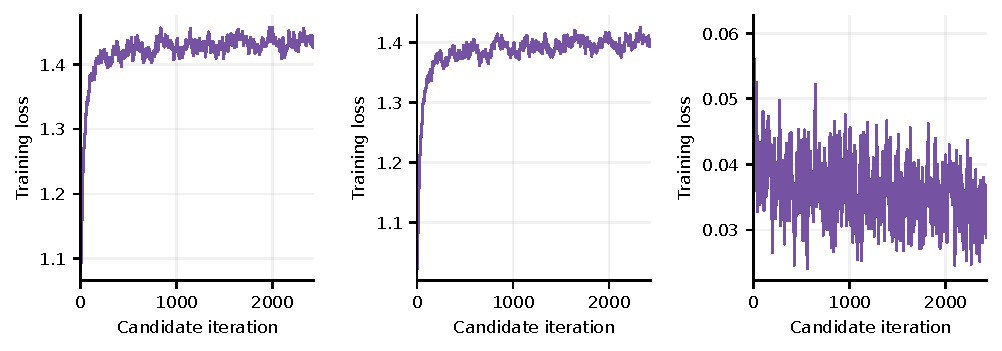
\includegraphics[width=\linewidth]{optimization.pdf}
\caption{Persistent/raw optimisation: final-epoch total loss, policy CE and value
MSE. Targets change during self-play; these are training diagnostics.}
\end{figure}
At the final candidate 2430 (raw iteration 2613), policy CE is 1.402395, value MSE is 0.029403, and total data loss is 1.431797.
These are online minibatch averages (Equation~\eqref{eq:logged-loss}),
separate from the fixed-set pilot losses.

\section{Items to Complete Before Final Submission}
\label{app:remaining}
The group still needs to verify member details, reflections and individual
GenAI disclosures. Review the Double DQN implementation, source archive and
agent demonstration, record the group presentation and complete the group
contribution form. Recheck the submission limits after final edits.

\clearpage
\section{Additional Empirical Diagnostics}
\label{app:diagnostics}
\path{evidence/benchmark-details.json} stores player-specific outcomes and hashes
of 232 worker records. All 3,712 games were replayed to verify legal moves and
terminal results. Diagnostic intervals use 50,000 opening-ID resamples with seed
20261118.

\begin{figure}[!htbp]
\centering
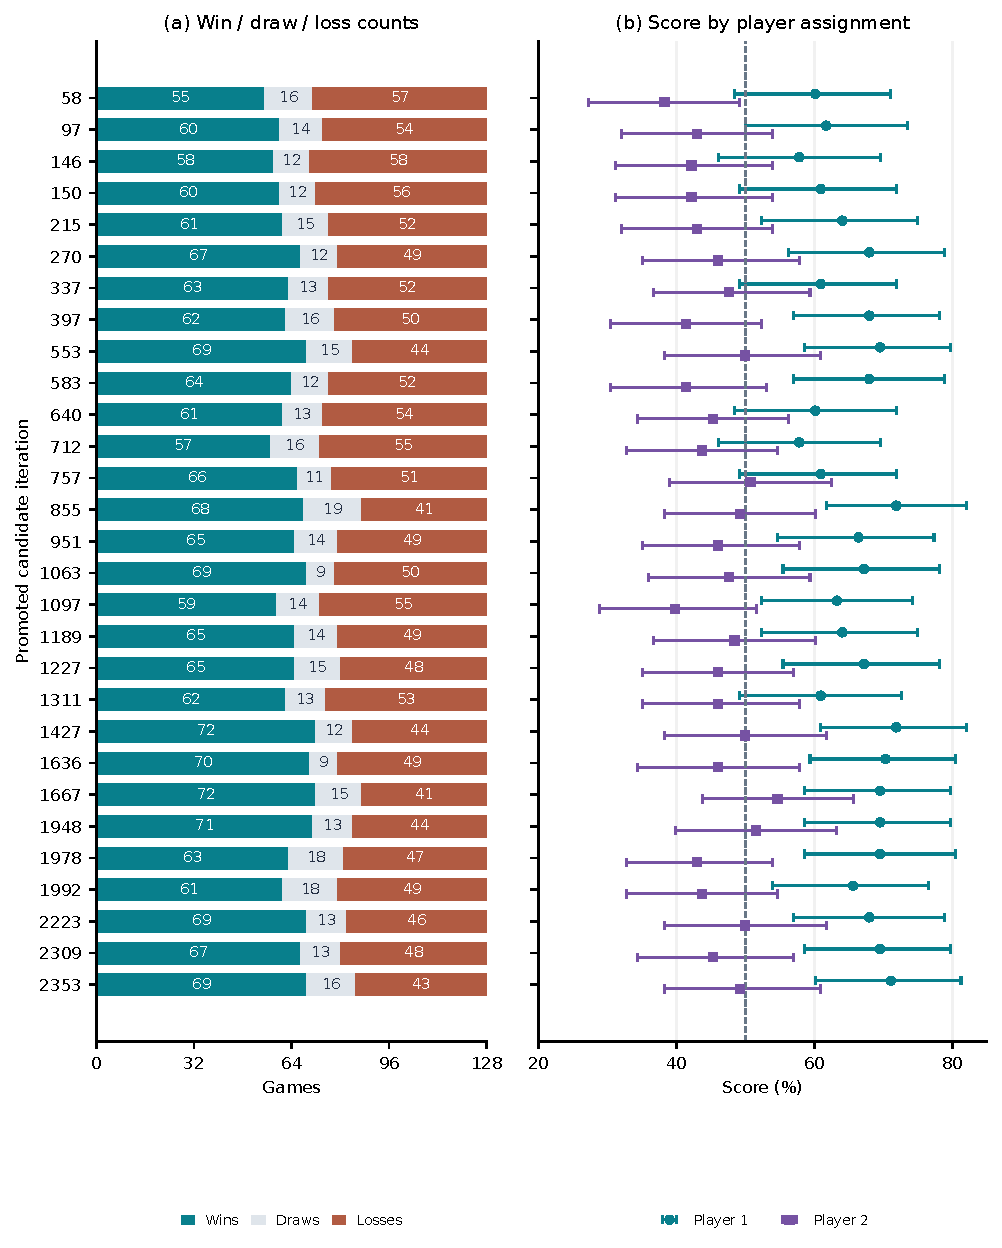
\includegraphics[width=\linewidth]{benchmark-outcomes.pdf}
\caption{Frozen-original outcomes: (a) win/draw/loss counts; (b) scores by player
assignment with pointwise 95\% intervals. Each assignment has 64 games; all
opening prefixes have even length.}
\label{fig:benchmark-outcomes}
\end{figure}

Candidate 2353 scored 71.1\% as player 1 and 49.2\% as player 2. Candidate 1667 scored 69.5\% and 54.7\%, respectively.

\begin{figure}[!htbp]
\centering
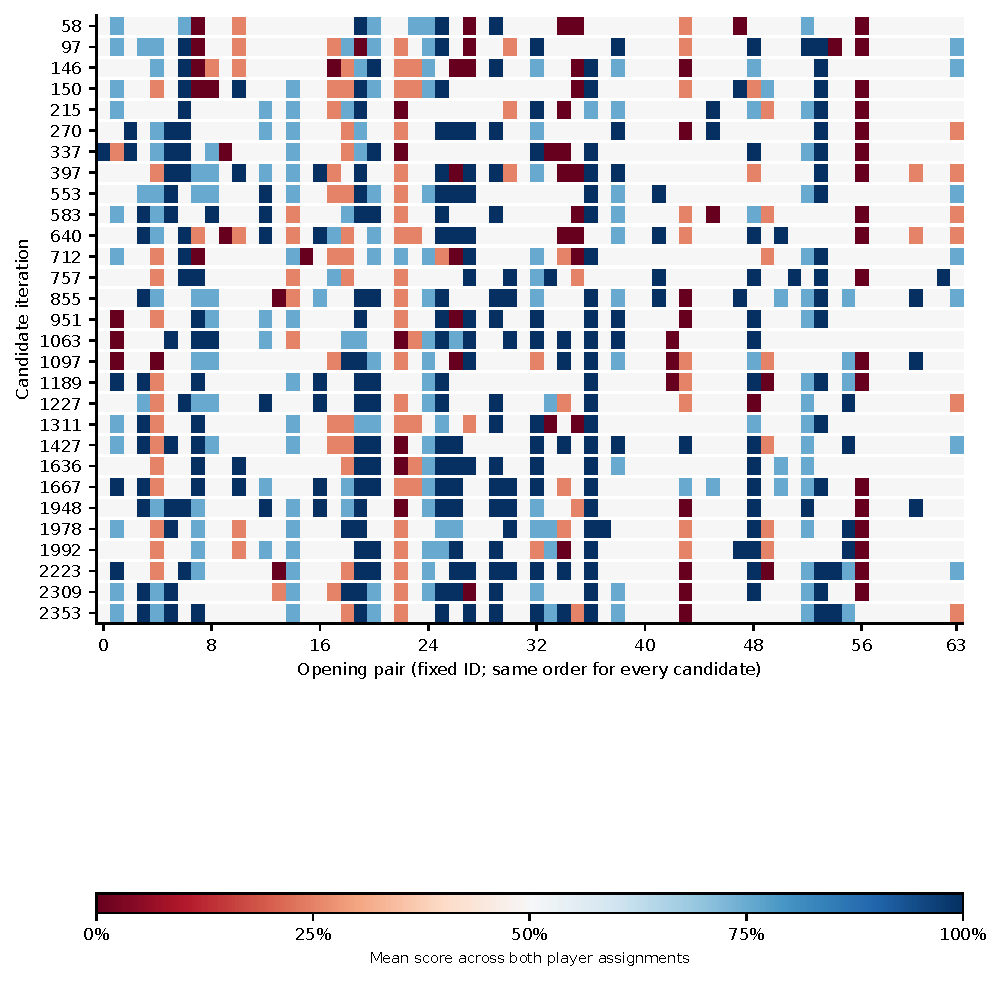
\includegraphics[width=\linewidth]{opening-performance.pdf}
\caption{Score per opening pair against the frozen original. Columns share
opening IDs across models; ID 0 is the empty board. A 50\% cell represents a
win/loss pair or two draws.}
\label{fig:opening-performance}
\end{figure}

\clearpage
\begin{figure}[!htbp]
\centering
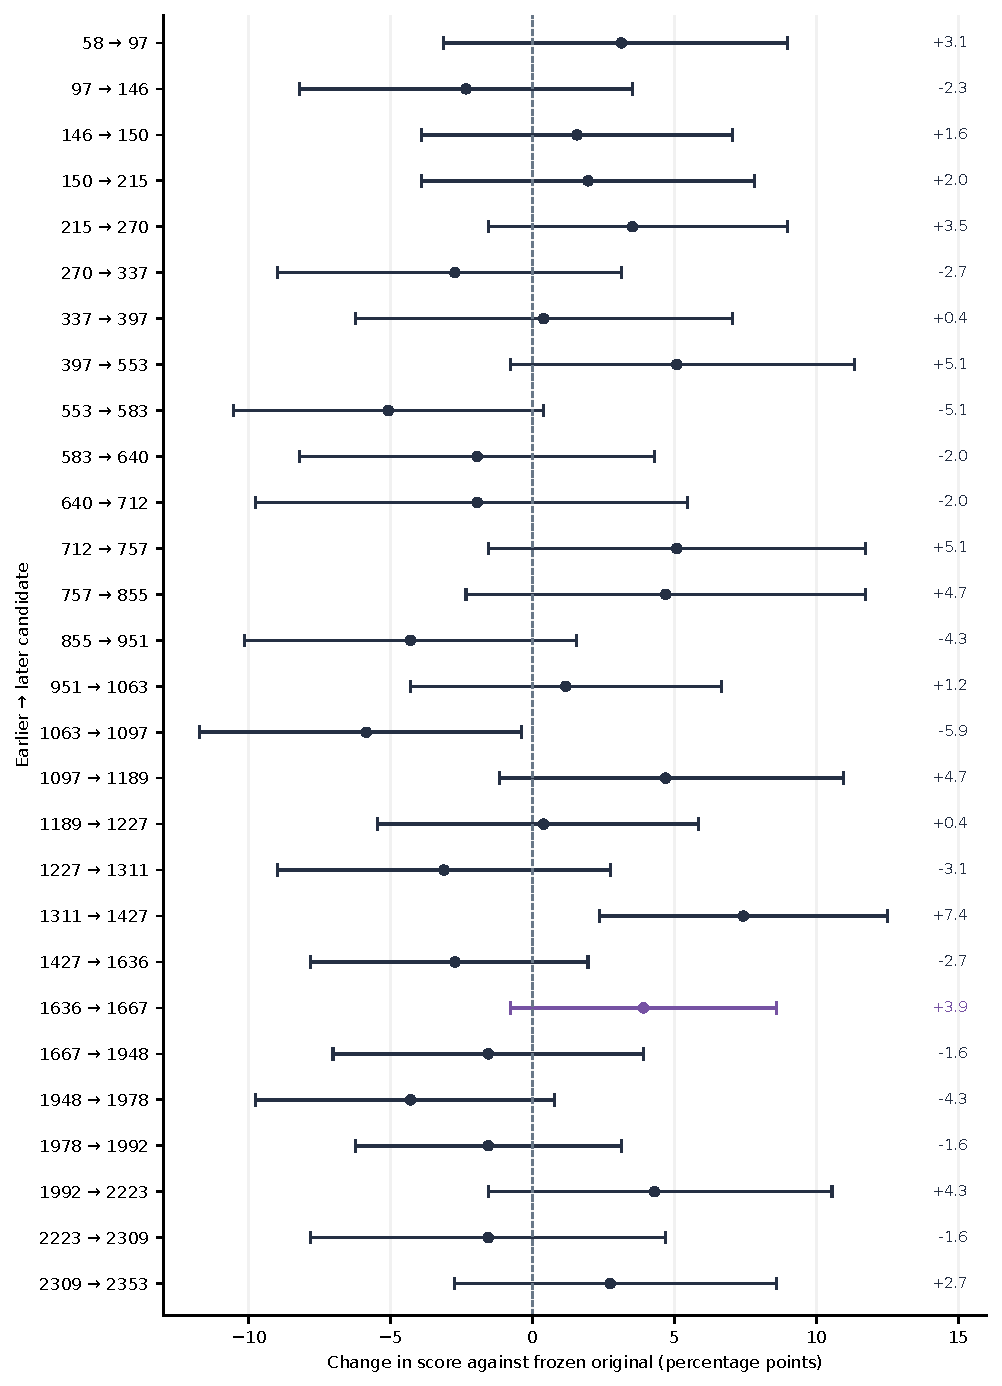
\includegraphics[width=\linewidth]{paired-improvements.pdf}
\caption{Change in fixed-original score between successive tested champions.
Pointwise 95\% intervals resample the 64 matched opening-pair differences.}
\label{fig:paired-improvements}
\end{figure}

26 of the 28 adjacent-difference intervals include zero. From candidate 2309 to 2353, the score changed by $+2.7$ percentage points (95\% interval $[-2.7, 8.6]$). The calculation preserves shared-opening dependence (Appendix~\ref{app:evaluation-math}). Intervals are pointwise across repeated comparisons.

\begin{figure}[!htbp]
\centering
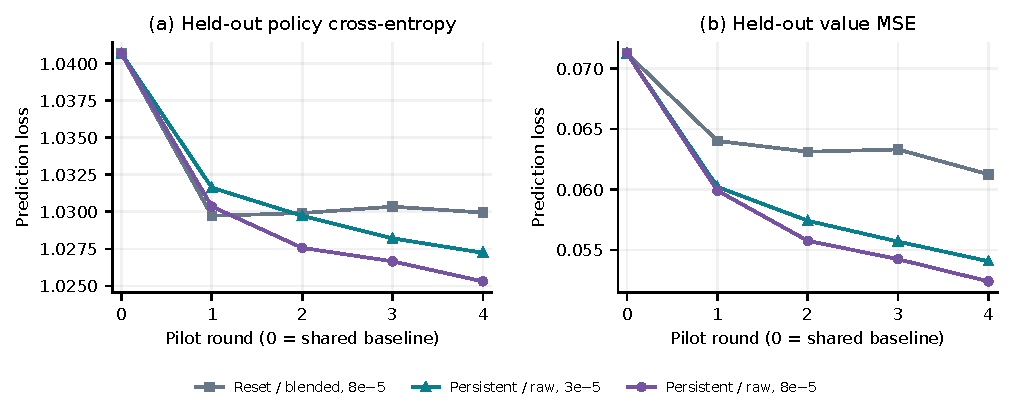
\includegraphics[width=\linewidth]{pilot-learning.pdf}
\caption{Pilot losses on 384 fixed withheld games plus reflections. Round 0 is
the shared starting model; each protocol has one continuation run.}
\label{fig:pilot-learning}
\end{figure}

Persistent/raw $8\times10^{-5}$ finishes with the lowest fixed-set losses
(Table~\ref{tab:pilot}). These curves compare prediction, while playing strength
is measured separately by games.

\clearpage
\section{Development Pilot for Double DQN}
\label{sec:ddqn-pilot}
We trained seed 51 from fresh weights for 5,000 games on Weatherwax
(86,076 moves and 21,264 updates). At game 0 and every
1,000 games, the greedy network played 32 fixed openings in both seats per
opponent. Each checkpoint used the same openings and random-opponent seeds.

Against uniform random play, score changed from 76.6\% to 95.3\% (61/0/3 wins/draws/losses at 5,000 games). The paired change was +18.8 percentage points (95\% interval [+7.8, +31.2]).

Against depth-two minimax, score changed from 0.8\% to 6.2\% (4/0/60 wins/draws/losses at 5,000 games). The paired change was +5.5 percentage points (95\% interval [+0.8, +10.9]).

The pilot provides evidence of improvement against uniform random play and depth-two minimax for this seed. Figure~\ref{fig:ddqn-pilot} shows the full trajectory.
The intervals quantify variation across the development opening pairs.
The matched study in Section~\ref{sec:q-study} addresses these limitations.

\begin{figure}[!htbp]
\centering
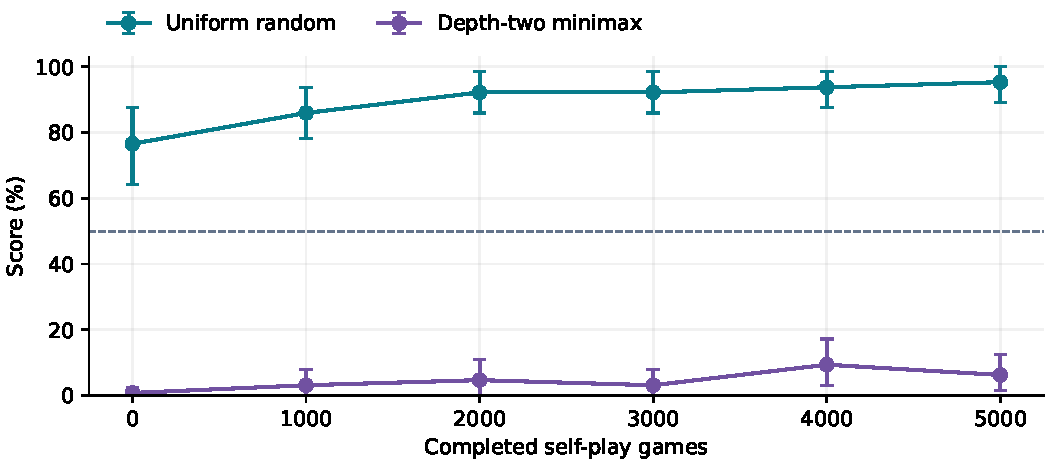
\includegraphics[width=\linewidth]{ddqn-pilot.pdf}
\caption{Double DQN from random weights. Each point uses 64 games against
the indicated opponent. Whiskers are pointwise paired-opening 95\% bootstrap
intervals across 32 openings, conditional on training seed 51.}
\label{fig:ddqn-pilot}
\end{figure}


\clearpage
\section{Matched Q-Learning Results}
\label{app:q-study}
\subsection{Learning curves and final scores}
\label{sec:q-study}
The seed-51 pilot identified missed immediate defences (Appendix~\ref{sec:ddqn-pilot}).
We then compared three matched initialisations on two fixed opponents.
Figure~\ref{fig:q-study} shows the learning curves for greedy inference.
On the fresh final openings, DQN and Double DQN changed by +24.5 and +24.7 percentage points against random play and by +10.4 and +10.2 points against minimax, respectively. The three paired Double DQN minus DQN differences against minimax were -2.3, +3.1, -1.6 points. The pairs do not establish a consistent advantage for either target rule. Table~\ref{tab:q-final} compares final inference variants.


\begin{table}[!htbp]
\centering\small
\caption{Mean score on 64 held-out opening pairs per seed, evaluated in both
seats. Learned variants use the 5,000-game checkpoint. Tactics only is the
shared reference for all seeds.}
\label{tab:q-final}
\begin{tabular}{@{}lrr@{}}
\toprule
Agent & Uniform random & Depth-two minimax\\
\midrule
Random weights & 70.3\% & 0.5\%\\
Random weights + guard & 90.4\% & 12.9\%\\
DQN & 94.8\% & 10.9\%\\
DQN + guard & 96.6\% & 27.2\%\\
Double DQN & 95.1\% & 10.7\%\\
Double DQN + guard & 97.4\% & 27.2\%\\
Tactics only & 90.6\% & 18.8\%\\
\bottomrule
\end{tabular}
\end{table}

DQN and Double DQN shared bit-identical initial weights within each seed.
The 32 learning-curve openings and 64 held-out openings were generated with
seeds 621903 and 736401. We excluded all pilot board positions from both sets
and all learning-curve positions from the held-out set. Each comparison uses
the same opponent, seat and opening across agents. Random opponent streams
are keyed by opening and seat. The 5,000-game checkpoint was fixed before
evaluation. We use a shared tactics-only control whose selection is uniform
within the filtered set.

\begin{table}[!htbp]
\centering\small
\caption{Per-seed held-out final scores. Each opponent plays 128 games against
each variant. Raw is the greedy network and guard adds the tactical filter.}
\begin{tabular}{@{}llrrrrrr@{}}
\toprule
Seed & Method & Moves & Updates & \multicolumn{2}{c}{Random} & \multicolumn{2}{c}{Minimax}\\
\cmidrule(lr){5-6}\cmidrule(l){7-8}
 & & & & Raw & Guard & Raw & Guard\\
\midrule
51 & DQN & 87,183 & 21,540 & 93.0\% & 96.1\% & 10.9\% & 27.0\%\\
51 & Double DQN & 86,076 & 21,264 & 95.3\% & 97.7\% & 8.6\% & 23.8\%\\
52 & DQN & 88,596 & 21,894 & 95.3\% & 96.9\% & 10.2\% & 27.0\%\\
52 & Double DQN & 87,274 & 21,563 & 96.9\% & 96.9\% & 13.3\% & 30.5\%\\
53 & DQN & 87,422 & 21,600 & 96.1\% & 96.9\% & 11.7\% & 27.7\%\\
53 & Double DQN & 90,459 & 22,359 & 93.0\% & 97.7\% & 10.2\% & 27.3\%\\
\bottomrule
\end{tabular}
\end{table}

We replayed all 11,008 evaluation games to verify legality and terminal
outcomes, and checked that filtered moves obeyed the tactical rule. Conditional
bootstrap intervals in the archive resample the same opening indices across
all runs and preserve the pairing between inference modes. They quantify
opening variation for the trained checkpoints. The archive
includes exact checkpoints, source, configurations and match histories.
The reported variation across training runs is based on three independent
initialisation pairs. Games within a run share weights and opening pairs.

\clearpage
\section{Move-Matched Tactics Study}
\label{app:tactical-study}
A certified losing move has successor $s'$ with an opponent winning reply.
The minimax value $V^*(s')$ is then $+1$, since the opponent can achieve
the maximum terminal payoff immediately. The mover's action value is
$-V^*(s')=-1$. An action surviving one reply has unknown exact value. The
computable set $C(s)$ therefore supplies sound partial supervision for
Eq.~\eqref{eq:tactical-loss}. The experiment does not modify exploration
or use the filter during data collection.

The curve, final and endgame generators use seeds 417507, 295813 and
563829. Evaluation boards are pairwise disjoint up to horizontal reflection,
and exclude 121 earlier boards up to reflection. The frozen test pack
records legal prefixes and action values. From live random prefixes with
8--12 empty cells, it selects positions with distinct legal outcomes.
The multi-step stratum admits no certified action. A memoised negamax
recursion obtains all remaining values and an independent column-grid
implementation verifies all 288 labels. Score is invariant to which
optimal action is chosen. We also report value regret
$\max_aQ^*(s,a)-Q^*(s,\hat a)$ in the source evidence.

\begin{table}[!htbp]
\centering\small
\caption{Primary final test by seed. Each run uses 80,000 moves and 19,745 updates. Final games vary in length and the budget can end during a game. The final column shows tactical minus plain in percentage points.}
\label{tab:tactical-seeds}
\begin{tabular}{@{}lrrrrr@{}}
\toprule
Seed & Games (plain) & Games (tact.) & Plain & Tactical & Diff. (pp)\\
\midrule
61 & 4,632 & 4,890 & 10.2\% & 10.2\% & +0.0\\
62 & 4,840 & 5,000 & 10.9\% & 10.9\% & +0.0\\
63 & 4,655 & 4,798 & 12.5\% & 10.2\% & -2.3\\
64 & 4,512 & 4,898 & 12.5\% & 9.4\% & -3.1\\
65 & 4,609 & 4,745 & 13.3\% & 8.6\% & -4.7\\
\bottomrule
\end{tabular}
\end{table}

The primary 95\% opening-pair bootstrap interval is [-4.2, +0.0] points. Its 20,000 resamples use common opening indices across seeds, preserving both seats. The paired $t$ interval instead uses the five seed-level differences. The primary comparison was fixed in the test pack before evaluation.

For the reflection ablation, we average $Q_\theta(s,a)$ with
$Q_\theta(Ms,6-a)$, where $M$ mirrors the board. This requires two network
evaluations. Inherited reference experiments use the same fixed
checkpoint for prior-only and 64-simulation PUCT, with no root noise.
They show the effect of search within that network on these positions.
Table~\ref{tab:tactical-oracle} reports the individual ablations.

\begin{table}[!htbp]
\centering\small
\caption{Optimal action rates on the solved set. Learned rows average five seeds. The inherited reference uses a separate network and search budget.}
\label{tab:tactical-oracle}
\begin{tabular}{@{}lrrr@{}}
\toprule
Policy & Win now & Defend & Multi-step\\
\midrule
Plain greedy & 78.8\% & 46.9\% & 53.1\%\\
Plain + guard & 100.0\% & 95.2\% & 53.1\%\\
Plain + mirror & 82.3\% & 52.7\% & 51.5\%\\
Tact. greedy & 81.5\% & 51.7\% & 50.8\%\\
Tact. + guard & 100.0\% & 95.2\% & 50.8\%\\
Tact. + mirror & 85.2\% & 56.5\% & 52.5\%\\
Inherited prior & 88.5\% & 97.9\% & 77.1\%\\
Inherited + PUCT & 100.0\% & 99.0\% & 93.8\%\\
\bottomrule
\end{tabular}
\end{table}

We validated all 10,400 match trajectories, including final rewards and filter compliance.
A score-preserving rerun restored traces after a recording-field collision. A separate replay checked all 2,496 lookahead matches. The archive contains checkpoints, source hashes, launchers, the frozen test pack and the replay analysis.

\section{Matched Controls for Horizon, Search and Defence}
\label{app:final-controls}

The original search and defence seeds are 61--65. The original horizon
seeds are 71--75. Each comparison adds seeds 81--85 on the same frozen
test sets. Each added seed starts three runs with identical weights
(plain one-step, tactical one-step and plain up to three steps).
The plain one-step training run serves all three comparisons, for 15
additional runs and 1,200,000 additional moves. The added-only summaries
separate replication from the original experiments. The contrasts share
trained runs, so their results can be correlated.

\subsection{Alternating multi-step returns}
Let $r_{t+j}$ be the reward to the mover at time $t+j$. Multiplying by
$(-1)^j$ expresses each reward in the perspective of the initial mover.
With $k$ realised steps, the Double DQN target is
\begin{equation}
 \begin{aligned}
 y_t^{(k)} &= \sum_{j=0}^{k-1} (-1)^j r_{t+j} + (-1)^k B(s_{t+k}),\\
 B(s) &= \begin{cases}
 Q_{\bar\theta}(s,\arg\max_{a\in\mathcal A(s)}Q_\theta(s,a)), & s\text{ live},\\
 0, & s\text{ terminal}.
 \end{cases}
 \end{aligned}
 \label{eq:multi-step}
\end{equation}
The last term is absent at terminal states. After an odd number of moves
the successor is the opponent. After an even number it is the initial
player again. Setting $k=1$ gives Eq.~\eqref{eq:ddqn}. For example, if the
opponent wins on the second move, the original mover's target is $0-1$.

The treatment takes $k\leq3$ and ends a sequence at termination, the
training budget, or before an intermediate action drawn by the
exploration branch. An exploratory action may start its own sequence.
This conservative Watkins-style cutoff~\cite{munos2016} reduces dependence
on exploratory replies. Replayed continuations can still be stale as the
network changes. This comparison tests the whole truncated-target rule
with function approximation. Both arms begin with identical weights
within a pair, share the architecture, exploration schedule and replay
capacity, and update on the same environment steps. Self-play trajectories
and completed game counts can differ. All weights at 80,000 moves are used.
The 20 runs in the horizon comparison completed 90,575 games across
1,600,000 moves. The treatment sampled 67.8\% one-step,
15.6\% two-step and 16.6\% three-step returns
over all updates. Counts include repeated replay samples.

\begin{table}[!htbp]
\centering\small
\caption{Greedy score and complete training games for the horizon control. Each final checkpoint faced depth-two minimax twice on each of 128 openings.}
\label{tab:horizon-seeds}
\begin{tabular}{@{}lrrrrr@{}}
\toprule
Seed & Games (one) & Games (up to three) & One & Up to three & Diff. (pp)\\
\midrule
71 & 4,504 & 4,317 & 11.3\% & 9.4\% & $-2.0$\\
72 & 4,506 & 4,600 & 10.9\% & 8.6\% & $-2.3$\\
73 & 4,491 & 4,556 & 10.9\% & 9.8\% & $-1.2$\\
74 & 4,394 & 4,597 & 10.5\% & 9.4\% & $-1.2$\\
75 & 4,588 & 4,409 & 10.5\% & 9.4\% & $-1.2$\\
\midrule
81 & 4,653 & 4,465 & 9.0\% & 10.9\% & $+2.0$\\
82 & 4,531 & 4,528 & 11.3\% & 10.4\% & $-1.0$\\
83 & 4,742 & 4,481 & 10.9\% & 11.3\% & $+0.4$\\
84 & 4,724 & 4,536 & 12.5\% & 9.8\% & $-2.7$\\
85 & 4,553 & 4,400 & 10.5\% & 8.6\% & $-2.0$\\
\bottomrule
\end{tabular}
\end{table}

\subsection{Leaf evaluator with a fixed two-ply tree}
For a legal root action the search takes the minimum over the opponent's
replies, then selects the action with maximum value. A terminal node
contributes the exact value to the root player even if it occurs before
two plies. At a live leaf $s''$ the root player moves again. We compare
\begin{equation}
 L_Q(s'')=\max_{c\in\mathcal A(s'')}Q_\theta(s'',c),\qquad
 L_H(s'')=\frac{H(s'')}{1+|H(s'')|}.
\end{equation}
Here $H$ is the minimax agent's score over board windows. The monotone
rescaling preserves its ordering and puts live leaves strictly between
terminal loss and win. Both variants use the same legal branches,
terminal shortcuts and ascending-column tie-break. The initial-weight
control keeps this tree and architecture with weights from step zero.
Guarded greedy uses the trained weights with one forward pass and the
immediate-win and safety filter. The shared heuristic baseline is one
deterministic policy. The depth-three opponent uses the same window
heuristic, so rankings are conditional on that benchmark.

The initial exploratory test used 24 opening pairs. The frozen follow-up
draws 128 pairs from random 2--10-ply non-terminal prefixes, excluding 521
previous evaluation positions up to reflection. These exclusions cover
the pilot, matched studies, earlier lookahead pack and solved positions.
They give a fresh opening set. Positions visited during self-play can
reappear in evaluation. We replayed all 13,056 games from the two cohorts,
checking opening and seat assignment, move legality and terminal rewards.

For each fixed checkpoint we play both seats and reduce them to one
score per opening. Pairing holds the seed and
opening IDs fixed when computing differences. The seed $t$ interval uses
ten seed differences on the frozen openings. The opening-pair bootstrap
resamples the 128 IDs jointly across policies and seeds. A crossed
bootstrap also resamples ten seed-pair IDs. Both use 20,000
draws~\cite{efron1979,agarwal2021}. The intervals are pointwise.
The sample SD uses $n-1$ in the denominator. For contrasts we compute a
difference within each seed before calculating its mean, SD and intervals.
The evidence file also reports the opening-only intervals.

\begin{table}[!htbp]
\centering\small
\caption{Paired score changes (mean $\pm$ SD) and 95\% intervals, in percentage points. The seed interval holds openings fixed. The joint interval varies training seeds and openings.}
\label{tab:control-intervals}
\begin{tabular}{@{}lrrrr@{}}
\toprule
Comparison & All ten & Added five & Seed interval & Joint interval\\
\midrule
Trained Q vs heuristic & $-9.0\pm1.7$ & $-9.3\pm1.5$ & $[-10.2,-7.8]$ & $[-14.2,-3.9]$\\
Trained Q vs initial Q & $+14.1\pm4.7$ & $+15.0\pm4.5$ & $[+10.7,+17.4]$ & $[+10.0,+17.9]$\\
Two-ply vs guarded Q & $+4.3\pm2.8$ & $+4.5\pm2.2$ & $[+2.3,+6.3]$ & $[+1.2,+7.4]$\\
Up to three vs one step & $-1.1\pm1.4$ & $-0.7\pm1.9$ & $[-2.1,-0.1]$ & $[-2.8,+0.5]$\\
\bottomrule
\end{tabular}
\end{table}

\subsection{Shared defensive positions}
We replayed the ten earlier greedy match sets and extracted boards before
ply 30 with both a move that allows an immediate opponent win and a move
that prevents it. We excluded positions with an immediate win for the
mover. The board set is fixed after removing duplicates up to reflection.
All 20 final Q-networks make decisions separately in both orientations.
We average outcomes across orientations with one decision per orientation.
The added seed pairs contributed no match trajectories to this board set. A move counts as an exposure
even if an imperfect opponent would fail to take its winning reply.

\begin{table}[!htbp]
\centering\small
\caption{Avoidable immediate loss on shared boards. Rates and paired differences (tactical minus plain, pp) show mean $\pm$ SD across ten seeds, or the five added seeds where indicated. Ply counts moves played.}
\label{tab:matched-defence}
\begin{tabular}{@{}lrrrr@{}}
\toprule
Position set & Boards & Plain & Tactical & Diff. (pp)\\
\midrule
All match boards & 1,797 & $(38.3\pm1.6)\%$ & $(42.9\pm1.4)\%$ & $+4.5\pm2.0$\\
Added seeds only & 1,797 & $(38.3\pm1.5)\%$ & $(43.5\pm1.1)\%$ & $+5.3\pm2.1$\\
Ply 0--9 & 52 & $(40.3\pm3.9)\%$ & $(44.7\pm6.3)\%$ & $+4.4\pm6.2$\\
Ply 10--19 & 1,322 & $(35.0\pm1.8)\%$ & $(38.9\pm1.5)\%$ & $+3.9\pm2.2$\\
Ply 20--29 & 423 & $(48.4\pm2.0)\%$ & $(54.9\pm1.6)\%$ & $+6.5\pm2.7$\\
Solved defence & 96 & $(49.0\pm4.8)\%$ & $(47.0\pm4.3)\%$ & $-2.0\pm4.9$\\
\bottomrule
\end{tabular}
\end{table}

The added seeds test the same positions with separately trained networks.
Their paired change is $+5.3\pm2.1$ points (95\% seed interval $[+2.7,+7.8]$).
For the original seeds, the positive gap persists after excluding each
pair's source boards. The solved defence row uses the same exposure
criterion on the 96 solved puzzles, with a 95\% seed interval of
$[-5.5,+1.6]$ points. Phase and solved-set results are
exploratory and conditional on the selected positions.

\clearpage
\section{Search-Agent Reference and Continued Training}
\label{app:search-study}
This experiment uses an inherited search agent and its fine-tuned
checkpoints. The persistent learner and internal gate help us track
continuation from the original weights. They are separate from the
independently implemented Q-learning comparison.

\subsection{Policy--value approximation and self-play}
The 1,843,144-parameter network takes three $6\times7$ binary planes: current-player
pieces, opponent pieces and player identity. A 128-channel stem feeds five
residual blocks with two $3\times3$ convolutions each~\cite{he2016}, using batch
normalisation and ReLU~\cite{ioffe2015}. Separate 32-channel heads produce seven
policy logits and a scalar value. The value head includes a 256-unit hidden layer
and tanh output (Figure~\ref{fig:inference}). Appendix~\ref{app:network-math} gives the full forward map and
parameter counts.


Self-play uses 512 MCTS simulations per move. With child values stored from the
child's player-to-move perspective, selection is
\begin{equation}
 a^*=\arg\max_{a\in\mathcal A(s)}
 \left[-Q(s_a)+c\,P(s,a)\frac{\sqrt{N(s)}}{1+N(s_a)}\right],\qquad c=2.
 \label{eq:puct}
\end{equation}
Here $s_a=T(s,a)$, $N$ counts visits, $Q$ is mean backed-up value (zero when
unvisited), and $P$ is the legal-action prior. Leaves use the network value or
exact terminal outcome; backup reverses signs between players.
Appendix~\ref{app:search-math} specifies the update.

Root noise has Dirichlet concentration 1.0 and mixture weight 0.15. With root
child counts $n_a=N(s_a)$, the stored target and move-sampling distribution are
\begin{equation}
 \pi(a\mid s)=\frac{n_a}{\sum_b n_b},\qquad
 \mu_\tau(a\mid s)=\frac{n_a^{1/\tau}}{\sum_b n_b^{1/\tau}}.
 \label{eq:visits}
\end{equation}
Temperature is 1.0 for the first 12 moves and 0.3 thereafter; it changes behaviour
but leaves raw visit targets intact. Each state receives its terminal outcome
$z$, and horizontal reflection adds a mirrored training example.

The network predicts $(p_\theta,v_\theta)$ and minimises
\begin{equation}
 \mathcal L(\theta)=\frac{1}{|\mathcal B|}\sum_{(s,\pi,z)\in\mathcal B}
 \left[-\sum_{a=0}^{6}\pi(a)\log p_\theta(a\mid s)
       +(v_\theta(s)-z)^2\right].
 \label{eq:data-loss}
\end{equation}
Training softmax includes all seven logits; search renormalises over legal
columns. Illegal actions have zero target mass but remain in the training
denominator (Appendix~\ref{app:loss-math}). Adam~\cite{kingma2015} uses learning
rate $8\times10^{-5}$, batches of 512, weight decay $10^{-5}$ and gradient norm
clipping at 1.0. BN running statistics are frozen; affine parameters remain
trainable. Appendix~\ref{app:optimiser-math} gives the exact update order.

Search supplies policy targets and sampled outcomes supply value targets. These
are fixed during regression, so gradients do not pass through search or games.
This approximates policy iteration~\cite{silver2018,anthony2017}; prediction loss
alone does not establish playing strength.

\subsection{Reset and persistent learning protocols}
The initial protocol restarted each candidate from the champion with a fresh
optimiser, training four epochs on the latest 16 shards of 64 games. Targets
blended search and teacher predictions:
$\tilde\pi=0.8\pi_{\mathrm{search}}+0.2p_{\mathrm{teacher}}$ and
$\tilde z=0.5z+0.5v_{\mathrm{teacher}}$, resembling distillation~\cite{hinton2015}.
Unsuccessful candidates lost their accumulated updates.

Persistent/raw training begins at candidate 0 (original log iteration 183).
A separate learner retains weights, Adam state and update count regardless of
promotion, and generates self-play with its latest weights. Each cycle trains
one epoch on raw targets from the latest 64 shards (4,096 games). Six GPU workers generate 384 games in a full cycle and share arena evaluation. The final cycle uses five generation workers and all six arena workers. Optimisation uses one GPU.
The champion remains a saved evaluation reference (Figure~\ref{fig:persistent-training})
(Appendix~\ref{app:replay-math}).

\begin{figure}[tbp]
\centering
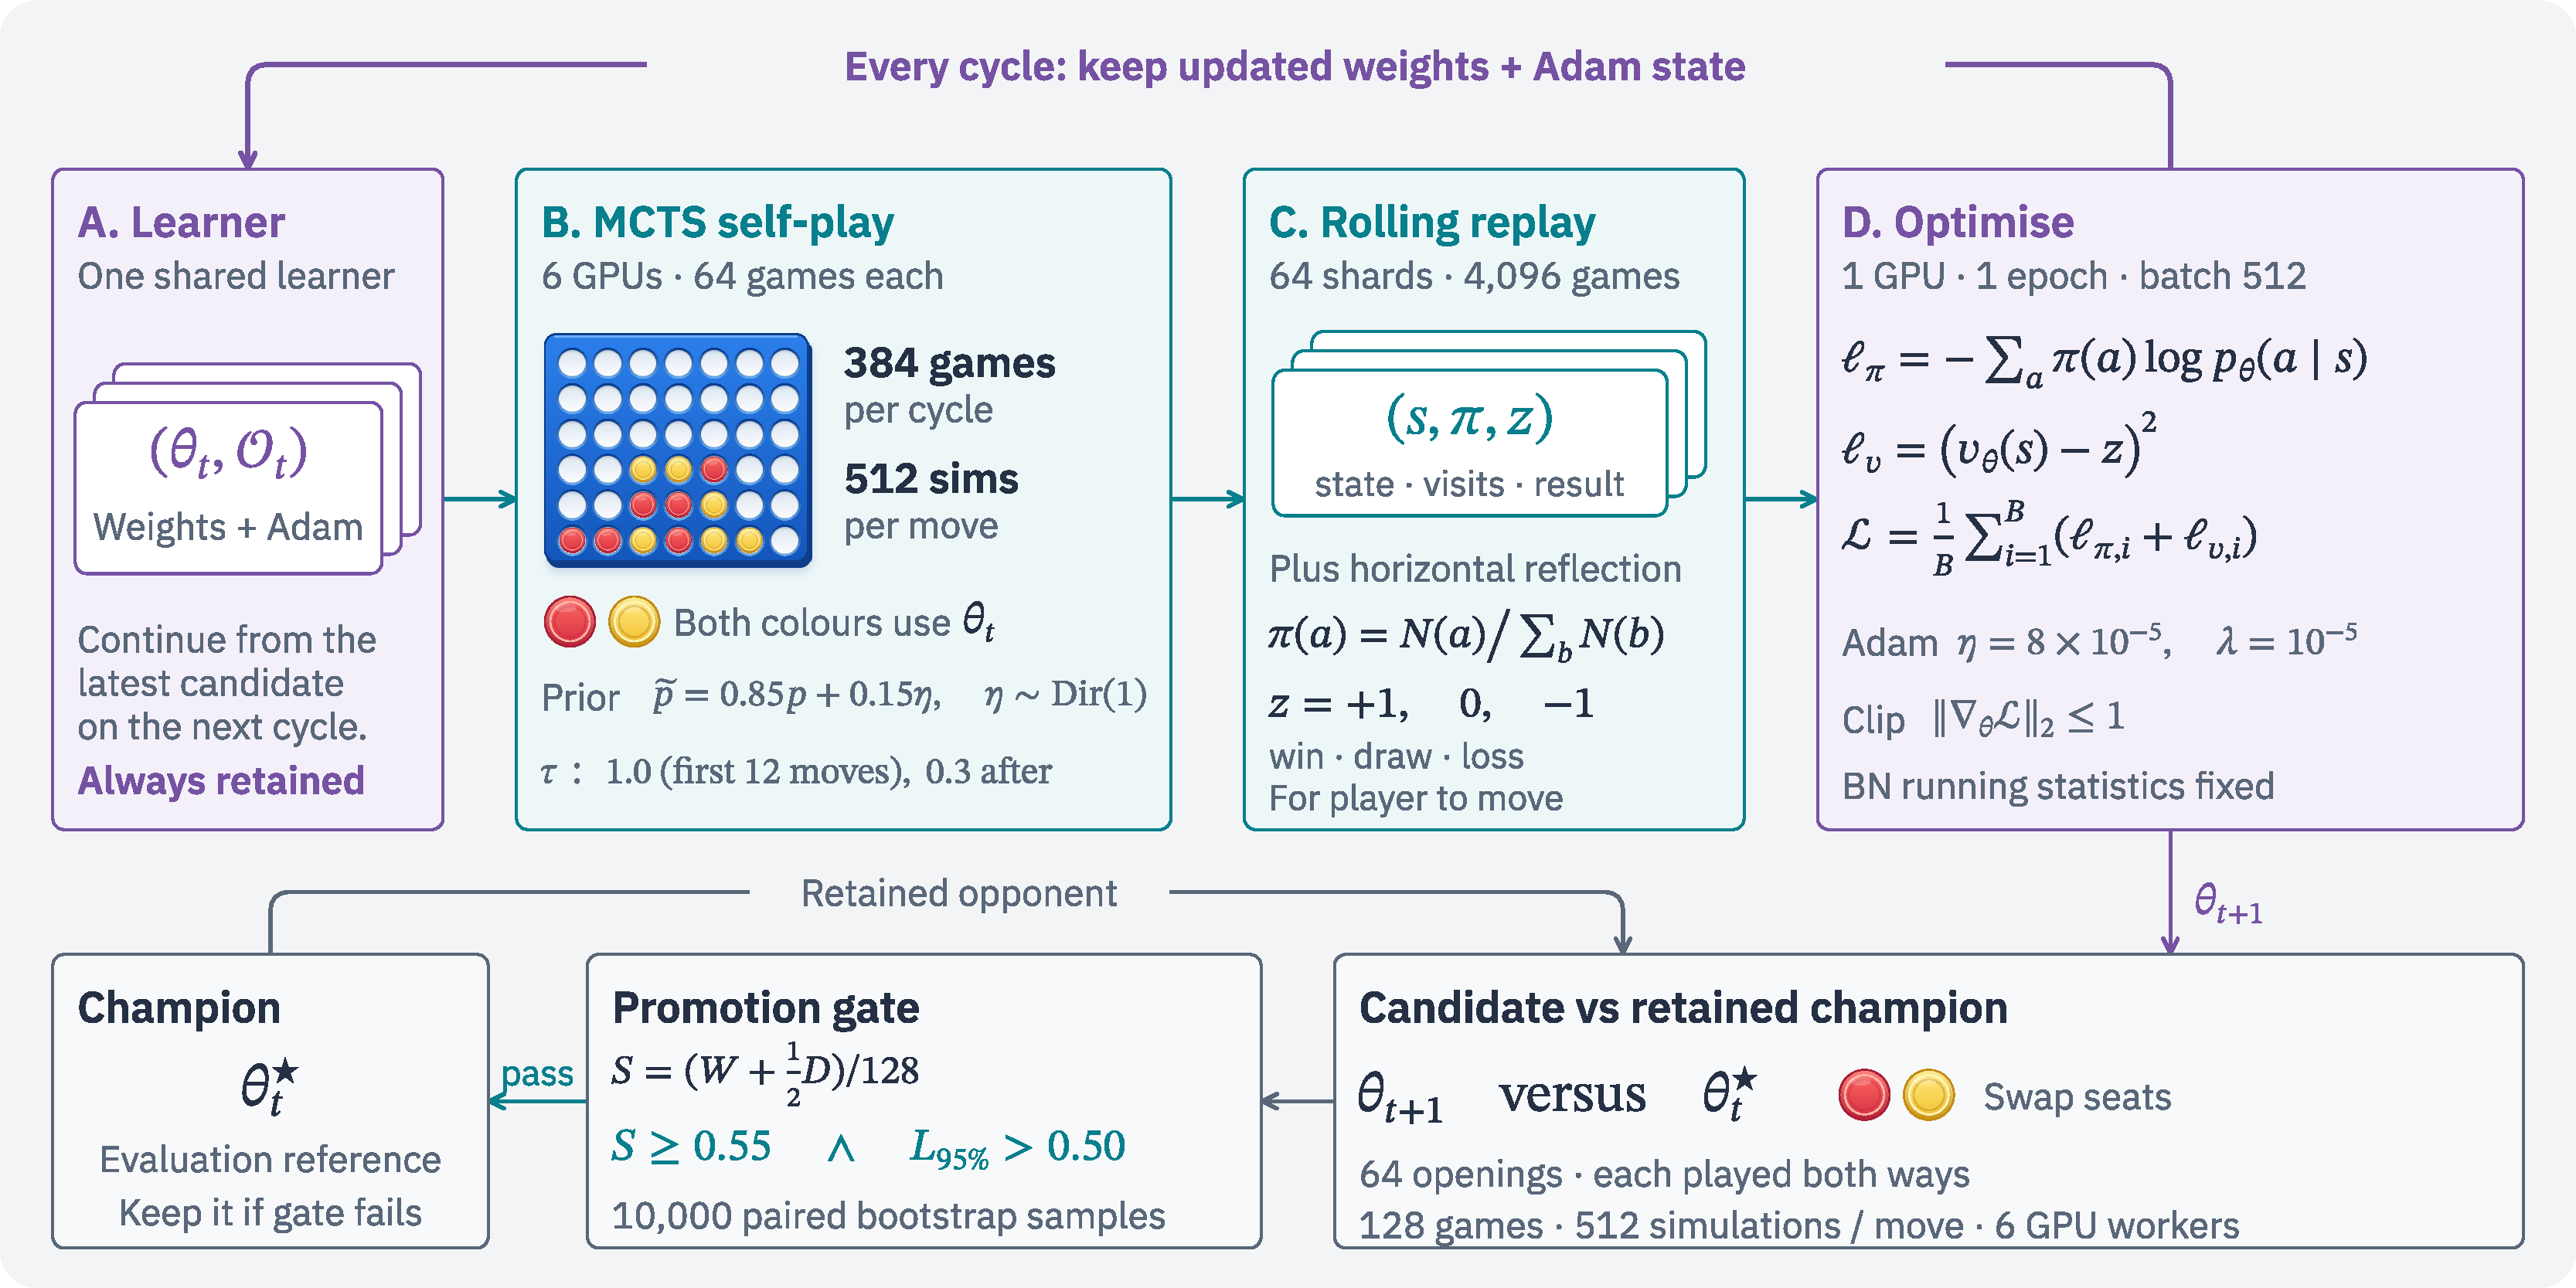
\includegraphics[width=\linewidth]{persistent-self-play.pdf}
\caption{Persistent training. Learner weights and Adam state survive every cycle;
the separate champion changes only after the promotion gate passes.}
\label{fig:persistent-training}
\end{figure}

A four-round pilot compared reset/blended at $8\times10^{-5}$ with persistent/raw
at $3\times10^{-5}$ and $8\times10^{-5}$, starting from the same champion and
historical data source. Prediction losses used six shared withheld shards
(384 games plus reflections); each final model played 128 arena games. Persistence,
targets, replay size and epochs changed together, so the pilot compares complete
protocols rather than individual components.

\subsection{Promotion and fixed-opponent evaluation}
An internal arena plays 64 distinct openings twice, swapping players, with
512-simulation budgets. Promotion requires score at least 55\% and paired 95\%
lower confidence bound above 50\%, using 10,000 bootstrap resamples. Workers
partition unique openings from candidate 0; earlier partitioning could duplicate them.

External benchmarks run exported agents against the same frozen original on
Weatherwax CPUs. Each model receives 128 games from the same 64 unique openings:
the empty board and non-terminal random legal prefixes of 2, 4, 6, 8 or 10 moves.
Both agents use identical code and configured 1.9-second budgets. Eight workers
occupy separate physical cores while training continues on the remaining cores.
Exported weights match checkpoints, and NumPy/PyTorch predictions are compared
on 40 positions. Deployment includes tactical checks and safety filtering absent
from the internal GPU arena.

We report score $S=(W+D/2)/n$. External 95\% intervals resample the 64 opening-pair
means 50,000 times, preserving both player assignments. They measure opening-level
variation, conditional on the trained models. Appendix~\ref{app:evaluation-math}
defines the estimators and their limitations.

\clearpage
\subsection{Protocol comparison}
All pilot settings reduce the shared baseline losses (policy CE 1.04068; value
MSE 0.07122). Persistent/raw at $8\times10^{-5}$ has the lowest final losses and
highest arena point estimate (Table~\ref{tab:pilot}); its fourth-round checkpoint
and Adam state seeded production. No setting passed the promotion gate, so this
was a provisional choice.

\begin{table}[htbp]
\centering\small
\caption{Four-round pilot: 128 arena games per setting, paired 95\% intervals,
and prediction losses on the same withheld data.}
\label{tab:pilot}
\begin{tabular}{@{}lrrrr@{}}
\toprule
Protocol / learning rate & Score & 95\% interval & Policy CE & Value MSE\\
\midrule
Reset/blended, $8\times10^{-5}$ & 48.8\% & 44.1--53.5\% & 1.02995 & 0.06125\\
Persistent/raw, $3\times10^{-5}$ & 51.2\% & 46.9--55.5\% & 1.02724 & 0.05407\\
Persistent/raw, $8\times10^{-5}$ & 53.1\% & 48.0--58.2\% & 1.02531 & 0.05241\\
\bottomrule
\end{tabular}
\end{table}

\subsection{Training progression and submission performance}
Training resumed from raw iteration 2,000 and produced 6 further promotions. Candidate 2353 finished as the retained champion after scoring 55.1\% against its predecessor (paired 95\% interval 50.4--59.8\%).

The 29 fixed-original tests comprise 3,712 games on the same 64 opening pairs. Candidate 2353 scored 60.2\% (69 wins, 16 draws and 43 losses, paired 95\% interval 54.7--66.0\%). The games recorded no invalid actions or moves over two seconds. Figure~\ref{fig:evaluation} shows the full benchmark series.

\end{document}
